%%
% The BIThesis Template for Bachelor Paper Translation
%
% 北京理工大学毕业设计(论文) —— 使用 XeLaTeX 编译
%
% Copyright 2020-2023 BITNP
%
% This work may be distributed and/or modified under the
% conditions of the LaTeX Project Public License, either version 1.3
% of this license or (at your option) any later version.
% The latest version of this license is in
%   http://www.latex-project.org/lppl.txt
% and version 1.3 or later is part of all distributions of LaTeX
% version 2005/12/01 or later.
%
% This work has the LPPL maintenance status `maintained'.
%
% The Current Maintainer of this work is Feng Kaiyu.
%
% Compile with: xelatex -> biber -> xelatex -> xelatex
%%

% !TeX program = xelatex
% !BIB program = biber


\documentclass[type=bachelor_translation]{bithesis}

\BITSetup{
  cover = {
    % 在封面中载入有「北京理工大学」字样的图片,如无必要请勿改动。
    headerImage = images/header.png,
    % 在封面标题中使用思源黑体,使用此选项可以保证与 Word 封面标题的字体一致。
    xiheiFont = STXIHEI.TTF,
    % 官方模板采用了固定的下划线宽度。我们采用以下两个选项来达成这个效果。
    % 如果你想要使用自动计算的下划线宽度,也可以删去以下两个选项。
    autoWidth = false,
    valueMaxWidth = 20em,
  },
  info = {
    title = 基于深度学习的端到端多实例点云配准,
    titleEn = {Deep Learning Based End-To-End \\ Multi-instance Point Cloud Registration},
    % 想要删除某项封面信息,直接删除该项即可。
    % 想要让某项封面信息留空(但是保留下划线),请设置为空字符串。
    % 如需要换行,则用 “\\” 符号分割。
    school = 自动化学院,
    major = 自动化,
    author = 杨润一,
    class = 06011902,
    studentId = 1120191211,
    supervisor = 由育阳,
    translationTitle = 多实例点云配准的高效对应聚类方法,
    translationOriginTitle = Multi-instance Point Cloud Registration \\ by Efficient Correspondence Clustering,
    keywords = {点云配准; 多实例; 聚类; 对应聚类; 深度学习;毕业设计(外文翻译)},
    % 如果你的毕设为校外毕设,请将下面这一行语句解除注释(删除第一个百分号字符)并填写你的校外毕设导师名字
  },
  style = {
    % 保持参考文献的缩进样式与 Word 模板一致。
    % 如果你不需要此样式,请将此行注释掉。
    bibliographyIndent = false,
    % head = {自定义页眉文字}
  }
}

% 有关参考文献的样式可以在此处修改;如无必要无需修改。
\usepackage[
  backend=biber,
  style=gb7714-2015,
  gbalign=gb7714-2015,
  gbnamefmt=lowercase,
  gbpub=false,
  doi=false,
  url=false,
  eprint=false,
  isbn=false,
]{biblatex}

\usepackage{caption}
\usepackage{subcaption}
\usepackage{graphicx}
\usepackage{amsmath}
\usepackage{amssymb}
\usepackage{amsfonts}
\usepackage{booktabs}
\usepackage{gensymb}


% 参考文献引用文件位于 misc/ref.bib
\addbibresource{misc/ref.bib}

% 文档开始
\begin{document}

% 标题页面:如无特殊需要,本部分无需改动
% \input{misc/0_cover.tex}
\MakeCover

% 前置页面定义
\frontmatter
%%%
% The BIThesis Template for Bachelor Graduation Thesis
%
% 北京理工大学毕业设计(论文)原创性声明模板 —— 使用 XeLaTeX 编译
%
% Copyright 2020-2023 BITNP
%
% This work may be distributed and/or modified under the
% conditions of the LaTeX Project Public License, either version 1.3
% of this license or (at your option) any later version.
% The latest version of this license is in
%   http://www.latex-project.org/lppl.txt
% and version 1.3 or later is part of all distributions of LaTeX
% version 2005/12/01 or later.
%
% This work has the LPPL maintenance status `maintained'.
%
% The Current Maintainer of this work is Feng Kaiyu.
%
% Compile with: xelatex -> biber -> xelatex -> xelatex
%
% 如无特殊需要,本页面无需更改

\MakeOriginality

% 摘要:在摘要相应的 TeX 文件处进行摘要部分的撰写
%%
% The BIThesis Template for Bachelor Graduation Thesis
%
% 北京理工大学毕业设计(论文)中英文摘要 —— 使用 XeLaTeX 编译
%
% Copyright 2020-2023 BITNP
%
% This work may be distributed and/or modified under the
% conditions of the LaTeX Project Public License, either version 1.3
% of this license or (at your option) any later version.
% The latest version of this license is in
%   http://www.latex-project.org/lppl.txt
% and version 1.3 or later is part of all distributions of LaTeX
% version 2005/12/01 or later.
%
% This work has the LPPL maintenance status `maintained'.
%  
% The Current Maintainer of this work is Feng Kaiyu.

% 中英文摘要章节
\begin{abstract}
    三维点云配准是点云处理中的一项基本任务,其在机械臂、自动驾驶、自主运动机器人、即时定位与地图构建(Simultaneous Localization and Mapping,SLAM)等众多基于视觉方法的应用中起着关键的作用。随着人工智能、元宇宙、自动驾驶等技术的兴起,将深度学习应用于点云配准的工作已经日趋成熟。目前大多数点云配准任务研究主要集中在成对配准上。然而,在实际应用中,目标场景可能包含多个重复实例,我们需要估计模板点云与目标点云中这些重复实例之间的多个刚性变换,也就是多实例点云配准。

    本文针对三维点云配准问题,特别是多实例点云配准,进行了深入研究。我们调研并整理了多实例点云配准的国内外研究现状,并总结了前人研究的优势和劣势。现有解决方案需要对大量假设进行采样以检测可能的实例并排除异常值,当实例和异常值的数量增加时,其鲁棒性和效率会显着降低。我们建议根据距离不变矩阵将噪声对应集直接分组到不同的簇中。通过聚类自动识别实例和异常值,达到稳健且快速表现。
    
    基于这一研究背景,我们提出了新的多实例点云配准架构,高效对应聚类的多实例点云配准 (ECC) 。分析聚类方法的点云配准,发现对于描述子的依赖性高,离群点比例高的时候效果会大大下降,所以我们提出了基于深度学习和聚类优化的多实例点云配准 (DMR),首先利用对比学习来学习输入推定对应关系的分布良好的深度表示。然后基于这些表示,我们提出了异常值修剪策略和聚类策略,以有效地删除异常值并将剩余的对应关系分配给正确的实例,达到了更好的效果。
    
    综上所述,我们的研究表明,基于深度学习的多实例点云配准方法在处理复杂的多实例点云配准问题上具有优秀的性能,提供了新的研究思路和方法。
    
\end{abstract}

% 英文摘要章节
\begin{abstractEn}
    Three-dimensional point cloud registration is a fundamental task in point cloud processing, which plays a crucial role in a wide range of vision-based applications such as robotic arms, autonomous driving, autonomous mobile robots, and Simultaneous Localization and Mapping (SLAM). With the rise of artificial intelligence, metaverse, autonomous driving, and other technologies, the application of deep learning to point cloud registration has become increasingly mature. Current research on point cloud registration mostly focuses on pairwise registration. However, in practical applications, the target scene may contain multiple repeated instances, and we need to estimate multiple rigid transformations between the template point cloud and these repeated instances in the target point cloud, that is, multi-instance point cloud registration.

    This paper conducts in-depth research on the problem of three-dimensional point cloud registration, especially multi-instance point cloud registration. We have surveyed and summarized the domestic and international research status of multi-instance point cloud registration and summarized the advantages and disadvantages of previous studies. Existing solutions require sampling a large number of hypotheses to detect possible instances and reject outliers, and their robustness and efficiency degrade significantly when the number of instances and outliers increases. We propose to directly group the noisy correspondence set into different clusters based on a distance invariance matrix. Through clustering, instances and outliers are automatically identified, achieving robust and fast performance.
    
    Based on this research background, we propose a new multi-instance point cloud registration framework, \textbf{E}fficient \textbf{C}orrespondence \textbf{C}lustering for Multi-instance Point Cloud Registration (\textbf{ECC}). After analyzing the point cloud registration of the clustering method, we find that the effect will drop significantly when it has high dependency on the descriptor and a high proportion of outliers. Therefore, we propose \textbf{D}eep Learning and Cluster Opimisation based \textbf{M}ulti-instance Point Cloud \textbf{R}egistration (\textbf{DMR}), which first uses contrastive learning to learn a good deep representation of the input estimation correspondence. Then, based on these representations, we propose an outlier pruning strategy and a clustering strategy to effectively remove outliers and allocate the remaining correspondences to the correct instances, achieving better results.
    
    In conclusion, our research shows that the deep learning-based multi-instance point cloud registration method has excellent performance in dealing with complex multi-instance point cloud registration problems and provides new research ideas and methods.
\end{abstractEn}

% 目录
\MakeTOC

% 正文开始
\mainmatter

% 第一章
%%
% The BIThesis Template for Bachelor Paper Translation
%
% 北京理工大学毕业设计(论文) —— 使用 XeLaTeX 编译
%
% Copyright 2020-2023 BITNP
%
% This work may be distributed and/or modified under the
% conditions of the LaTeX Project Public License, either version 1.3
% of this license or (at your option) any later version.
% The latest version of this license is in
%   http://www.latex-project.org/lppl.txt
% and version 1.3 or later is part of all distributions of LaTeX
% version 2005/12/01 or later.
%
% This work has the LPPL maintenance status `maintained'.
%
% The Current Maintainer of this work is Feng Kaiyu.
%
% Compile with: xelatex -> biber -> xelatex -> xelatex
%%

% 第一章节

\chapter{引言}

三维点云配准\cite{TEASER, DCP, paulj1992method}主要关注在源点云和目标点云之间估计一个单一的变换。然而,我们有时可能希望在点云之间估计多个变换。例如,我们有一个物体的3D扫描,可能希望在目标点云中找到如图\ref{fig:problem}所示的同一物体在桌子上的姿态。这个问题,我们称之为多实例点云配准,文献中较少研究。这个问题,我们称之为多实例点云配准,文献中较少研究。将现有的点云配准方法扩展到解决这个问题并非易事。

主要的挑战是在嘈杂的对应关系集合中识别属于不同实例的对应点的不同簇。一种解决方案是采用3D物体检测器或将实例分割应用于目标点云。然后,通过常规的点云配准方法估计每个实例的姿态。然而,这种方法需要为特定对象或类别训练检测器或分割网络\cite{VoteNet, Occuseg},不适用于未知对象或任意3D扫描。

\begin{figure}[htbp]
  \centering
  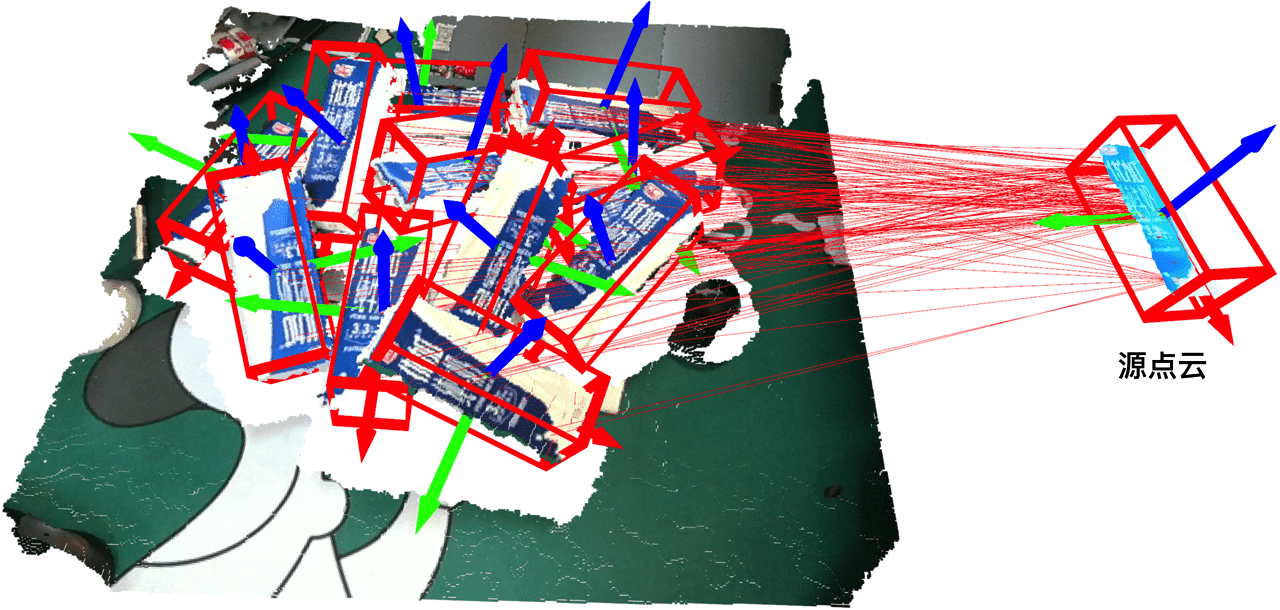
\includegraphics[width=0.8\textwidth]{images/problem.png}
  \caption{多实例点云配准:给定一个物体的源点云,多实例配准需要估计目标点云中每个物体的姿态。}
  \label{fig:problem} % label 用来在文中索引
  \vspace{-0.5in}
\end{figure}



另一种解决方案是通过多模型拟合\cite{Tlinkage, RPA, Coverage}或\cite{MCT, CONSAC, ProgressiveX2}。现有的多模型拟合方法依赖于采样有效的假设,当模型数量或异常值比例变高时,涉及大量的采样步骤,使得这些算法的效率和鲁棒性急剧下降。

在本文中,我们提出了一种鲁棒且高效的多实例三维配准问题解决方案。关键思想是根据距离不变性矩阵直接将对应点分组到不同的簇中。具体而言,在使用诸如D3Feat \cite{D3Feat}、PREDATOR \cite{PREDATOR}或SIFT \cite{lowe2004distinctive}等描述符进行特征匹配得到点对应关系之后,通过检查每对对应关系之间的距离一致性来构造矩阵。我们发现这个矩阵的行或列向量具有强大的表示能力,可以用于识别特定实例的对应关系集合。因此,我们应用了一种简单且高效的聚类算法将这些对应关系划分为团。通过将相似簇合并并重新分配簇id给每个对应关系,递归地进行几步细化聚类。最后,通过一个简单的排序策略自动识别每个实例的异常值和内点。



由于不需要耗时的假设采样,我们的方法具有很高的效率。我们在合成数据集和真实世界数据集上进行了广泛的实验。结果表明,我们的方法在准确性和鲁棒性方面表现明显优于现有方法,速度至少快10倍。总之,我们的贡献包括:
\begin{itemize}
\setlength{\itemsep}{-1pt}
\setlength{\parsep}{-2pt}
\item 我们提出了一种针对多实例点云配准问题的高效且鲁棒的解决方案,其在准确性、鲁棒性和速度方面都具有优越的性能。
\item 我们提出使用三个指标(平均命中召回率、平均命中精确度和平均命中F1)来全面评估多实例点云配准的性能。%据我们所知,尚未有针对这类评估的指标提出。
\item 我们的解决方案可以用于零样本检测3D物体,正如我们的真实世界测试所示。
\end{itemize}


% 在这里添加第二章、第三章……TeX 文件的引用
%%
% The BIThesis Template for Bachelor Paper Translation
%
% 北京理工大学毕业设计(论文) —— 使用 XeLaTeX 编译
%
% Copyright 2020-2023 BITNP
%
% This work may be distributed and/or modified under the
% conditions of the LaTeX Project Public License, either version 1.3
% of this license or (at your option) any later version.
% The latest version of this license is in
%   http://www.latex-project.org/lppl.txt
% and version 1.3 or later is part of all distributions of LaTeX
% version 2005/12/01 or later.
%
% This work has the LPPL maintenance status `maintained'.
%
% The Current Maintainer of this work is Feng Kaiyu.
%
% Compile with: xelatex -> biber -> xelatex -> xelatex
%%

% 第一章节

\chapter{相关工作}

\textbf{点云配准}可以分为三个阶段:点匹配、异常值剔除和姿态估计。大多数工作集中在前两个阶段,因为获得正确的点对应关系是成功配准的关键。点匹配通常依赖于特征,可以是手工设计的特征\cite{rusu2009fast, drost2010model},也可以是基于学习的特征\cite{3DMatch, PPFNet, 3DSmoothNet, FCGF, D3Feat}。尽管近期的结果显示,在某些基准测试中,后者优于手工设计的特征,但这些特征仍然无法实现完美匹配,因此仍然需要强大的异常值剔除机制。
RANSAC\cite{RANSAC}及其变体(\cite{GCRansac, NGRansac, LORansac})遵循假设-验证过程来剔除异常值。当存在许多异常值时,这类方法需要大量的采样步骤,耗时严重,而且仍可能无法获得正确的模型。GORE\cite{bustos2017guaranteed}和PMC\cite{parra2019practical}试图通过几何一致性检查来减少异常值。其他方法如FGR\cite{FGR}和TEASER\cite{TEASER}采用鲁棒估计器直接从噪声对应关系中解决变换问题。通过仔细处理每个子问题,TEASER\cite{TEASER}在鲁棒性和效率方面取得了令人印象深刻的性能。
还有一些基于学习的异常值剔除方法。DGR\cite{DGR}和3DRegNet\cite{3DRegNet}将异常值剔除视为二分类问题,并预测每个对应关系的内点概率。PointDSC\cite{PointDSC}进一步将空间一致性嵌入到特征学习中,以便更好地训练内点分类器。
最近,一系列工作(如PointNetLK\cite{PointNetLK},FMR\cite{FMR},DCP\cite{DCP},PRNet\cite{PRNet},RPMNet\cite{RPMNet})尝试将端到端学习应用于解决配准问题。它们在性能方面也表现出色,特别是在低重叠情况下\cite{PREDATOR}。

现有的点云配准方法主要关注一对一配准问题,即估计两个点云之间的单一变换。然而,将源点云与目标点云中的多个实例对齐的多实例配准问题则研究较少。这个任务与多路配准\cite{choi2015robust}不同,后者的目标是通过成对配准\cite{FGR}\cite{DGR}从多个片段生成全局一致的重建。多实例配准需要不仅从噪声对应关系中剔除异常值,还要识别出各个实例的内点集,使其比经典配准问题更具挑战性。

\textbf{3D目标检测和实例分割}与多实例3D配准密切相关。给定一个单独的点云,3D目标检测\cite{VoteNet}的目的是获取每个感兴趣对象的边界框,而3D实例分割\cite{SGPN, Occuseg}为每个点生成实例标签。尽管它们生成的结果\cite{avetisyan2019end, Scenecad}与多实例配准类似,但它们需要将特定对象或类别的先验训练到网络中。相比之下,多实例配准通过直接将源点云与目标点云中的多个实例对齐来处理两个点云,而不使用关于输入3D扫描内容的任何先验知识。

\textbf{多模型拟合}
多实例配准可以通过多模型拟合方法来解决,其目的是从多模型生成的数据点中估计模型参数。
% 例如,给定一组从不同线条或圆圈采样的2D点,多模型拟合的目的是估计每条线或圆圈的参数。
现有的多模型拟合方法可以分为基于聚类的方法和基于RANSAC的方法。基于聚类的方法(例如\cite{Tlinkage, RPA, Coverage})通过采样点初始化一个庞大的假设集,然后为每个点计算关于这些假设的偏好向量。根据它们的偏好向量对这些数据点进行聚类。最后,从不同的簇计算模型参数。基于RANSAC的方法(如\cite{PEARL, MultiX, ProgressiveX, MCT, CONSAC, ProgressiveX2})顺序运行修订后的RANSAC以获得多个模型参数。它们在每次迭代中改变每个点的采样权重以获得不同的模型参数。CONSAC\cite{CONSAC}是一种基于学习的方法,通过学习为每个点分配采样权重。无论是基于聚类的方法还是基于RANSAC的方法,都依赖于采样有效假设。当模型数量或异常值比例增加时,需要采样很多假设,这使得这些算法效率非常低。

\textbf{3D空间一致性}是3D配准中异常值剔除的重要属性,它在每对点之间通过刚性变换来定义。谱匹配\cite{leordeanu2005spectral}通过在每对对应关系之间使用长度一致性来构建一个图,并从图中提取最大团以剔除异常值。现有的方法如TEASER\cite{TEASER},GORE\cite{bustos2017guaranteed}和PMC\cite{parra2019practical}也将空间一致性纳入到它们的算法中。最近,ROBIN\cite{shi2021robin}将空间一致性的概念推广到更高阶。PointDSC\cite{PointDSC}将空间一致性集成到端到端学习管道中,以便更好地回归内点概率。

受这些工作的启发,我们也采用了空间一致性作为解决方案。与现有方法(如谱聚类\cite{leordeanu2005spectral}或近似解\cite{shi2021robin})在空间一致性图中应用的方法不同,这些方法速度较慢且难以处理多个实例,我们采用了一种高效的算法来在对应关系中找到多个实例。具体来说,我们将距离不变矩阵的行向量或列向量作为对应关系的“特征向量”,并运行自底向上的聚类来从不同实例中获得内点对应关系。我们的方法避免了假设采样,这是现有多模型拟合方法的关键弱点。它还不依赖于任何特定特征来获得点对应关系,因此,如果采用更好的特征(无论是3D特征还是图像特征),性能可以进一步提高。







%%
% The BIThesis Template for Bachelor Paper Translation
%
% 北京理工大学毕业设计(论文) —— 使用 XeLaTeX 编译
%
% Copyright 2020-2023 BITNP
%
% This work may be distributed and/or modified under the
% conditions of the LaTeX Project Public License, either version 1.3
% of this license or (at your option) any later version.
% The latest version of this license is in
%   http://www.latex-project.org/lppl.txt
% and version 1.3 or later is part of all distributions of LaTeX
% version 2005/12/01 or later.
%
% This work has the LPPL maintenance status `maintained'.
%
% The Current Maintainer of this work is Feng Kaiyu.
%
% Compile with: xelatex -> biber -> xelatex -> xelatex
%%

% 第一章节

\chapter{问题陈述}


在多实例点云配准问题中,源点云$\mathbf{X}$提供了一个3D模型的实例,目标点云$\mathbf{Y}$包含了这个模型的$K$个实例,其中这些实例是一组点的集合,这些点可能只采样了3D模型的一部分。如果我们将第$k^{th}$个实例写为$\mathbf{Y}_k$,那么目标点云$\mathbf{Y}$可以分解为$
%\begin{equation}
\mathbf{Y} = \mathbf{Y}_0 \cup \mathbf{Y}_1 \cup \ldots \mathbf{Y}_k \ldots \cup \mathbf{Y}_K$。
%\end{equation}
这里我们使用$\mathbf{Y}_0$表示点云中不属于任何实例的部分。
多实例3D配准的目标是找到刚性变换$(\mathbf{R}_k, \mathbf{t}_k)$,将源实例$\mathbf{X}$对准到每个目标实例$\mathbf{Y}_k$。
如果我们设法获得源实例与每个目标实例$\mathbf{X} \leftrightarrow \mathbf{Y}_k$之间的对应关系,那么通过最小化对齐误差之和(\ref{eq:solve_rigid_transform}) \cite{SVD},可以从对应关系集合$\mathbf{X}\leftrightarrow \mathbf{Y}_k$中求解目标点云中第$k^{th}$个实例的位姿$(\mathbf{R}_k, \mathbf{t}_k)$:
\begin{equation}
\underset{\mathbf{R}_k,\mathbf{t}k}{\min}\sum_i{\parallel}\mathbf{y}{ki}-(\mathbf{R}_k\mathbf{x}_i+\mathbf{t}_k)\parallel ^2.
\label{eq:solve_rigid_transform}
\end{equation}
考虑到我们已经获得了源点云和目标点云之间的一组对应关系$\mathcal{C}$。多实例配准任务的关键是将这些对应关系分类为与不同实例相关的独立集合,即:
\begin{equation}
\mathcal{C} = \mathcal{C}_0 \cup \mathcal{C}_1\cdots \cup \mathcal{C}_K.
\end{equation}
这里,$\mathcal{C}_0$用来表示异常值集合。如我们所见,多实例配准不仅需要剔除异常值对应关系,还需要解决来自不同实例的对应关系的歧义。这个任务并不容易,因为所有实例看起来都一样,而且通常存在大量的异常值对应关系。











%%
% The BIThesis Template for Bachelor Paper Translation
%
% 北京理工大学毕业设计(论文) —— 使用 XeLaTeX 编译
%
% Copyright 2020-2023 BITNP
%
% This work may be distributed and/or modified under the
% conditions of the LaTeX Project Public License, either version 1.3
% of this license or (at your option) any later version.
% The latest version of this license is in
%   http://www.latex-project.org/lppl.txt
% and version 1.3 or later is part of all distributions of LaTeX
% version 2005/12/01 or later.
%
% This work has the LPPL maintenance status `maintained'.
%
% The Current Maintainer of this work is Feng Kaiyu.
%
% Compile with: xelatex -> biber -> xelatex -> xelatex
%%

% 第一章节

\chapter{方法}

我们提出的方法的概述如图\ref{fig:pipeline}所示。我们的方法以点对应关系作为输入。接着通过检查对应关系之间的距离一致性来构建一个不变性一致性矩阵。然后,通过将列或行向量视为这些对应关系的“特征”,将这些对应关系快速聚类成不同的组。通过凝聚聚类方法高效地进行聚类,然后通过交替合并相似的变换和重新分配簇标签进行多次迭代来进一步优化。在对应关系数量较大的情况下,我们可以选择性地应用降采样和上采样过程。详细内容将在接下来的章节中介绍。

\begin{figure*}[ht]
    \centering
    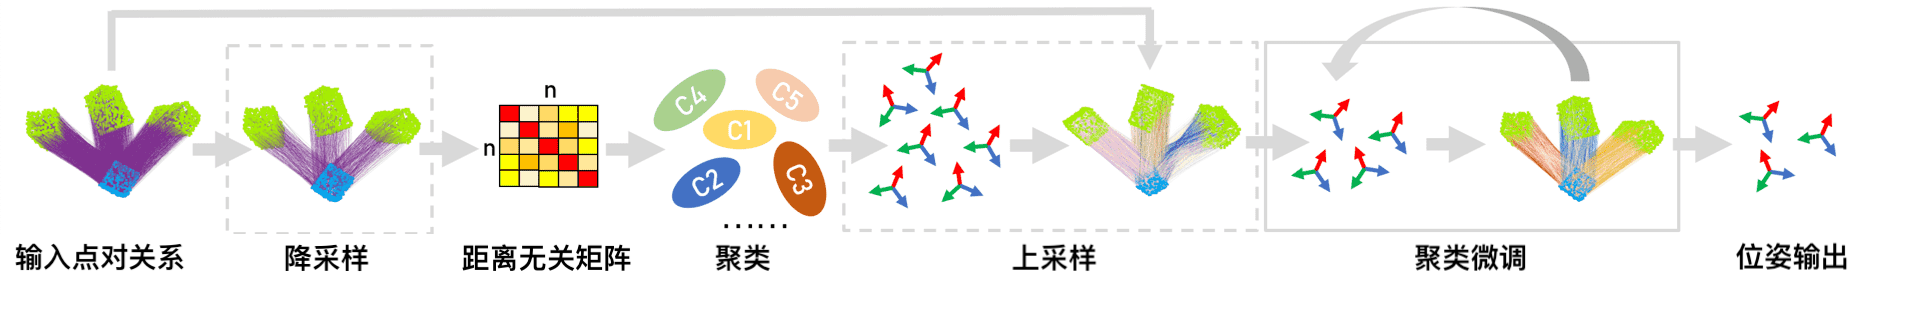
\includegraphics[width=1\textwidth]{images/pipeline.png} % Reduce the figure size so that it is slightly narrower than the column. Don't use precise values for figure width.This setup will avoid overfull boxes.
    \caption{我们提出的多实例点云配准方法的流程。从输入对应关系构建距离不变性矩阵,用于将对应关系聚类为不同的簇(\textbf{聚类}),并进行优化(\textbf{簇优化})。最后,从每个对应关系簇中估计与每个实例相关的刚体变换(\textbf{变换})。为了处理大量的对应关系,采用两个附加过程(\textbf{下采样}和\textbf{上采样})。}
    \label{fig:pipeline}
    \vspace{-0.6in}
\end{figure*}

\section{不变性矩阵和兼容性向量}
\label{subsec:Distance-Consistency-Graph}
距离不变性特性在3D配准领域已经被研究多年\cite{TEASER}\cite{shi2021robin}\cite{leordeanu2005spectral},该特性描述了在刚性变换之后两点之间的距离保持不变。具体来说,如果 $c_i :\mathbf{x}i \leftrightarrow \mathbf{y}i$ 和 $c_j : \mathbf{x}j \leftrightarrow \mathbf{y}j$ 是两个真实的对应关系,那么它们应该满足
%
\begin{equation}
G{ij}=|d{ij} - d'{ij} | < \delta
\label{eq:abs_diff}
\end{equation}
其中 $d{ij} = |\mathbf{x}i-\mathbf{x}j|, d'{ij}=|\mathbf{y}i -\mathbf{y}j|$,$\delta $ 是一个用于考虑噪声的阈值。
因此,$d{ij}$ 和 $d'{ij}$ 之间的差异可以用作度量是否存在异常值,或者两个对应关系是否来自不同的刚性变换的指标。我们参考\cite{matrix},使用相对差异作为度量,而不是在(\ref{eq:abs_diff})中定义的绝对差异,
\begin{equation}
G{ij} = s_{ij}^2, s_{ij} = \min( \frac{d_{ij}}{d'{ij}}, \frac{d'{ij}}{d_{ij}}) \in (0, 1).
\end{equation}
通过计算所有对应关系对之间的分数,可以获得一个\emph{距离不变性矩阵} $G$(我们令 $G_{ii} = 1$)。距离不变性矩阵是对称的,其中每一列或行是一个向量,描述了给定对应关系与其他对应关系之间的兼容性\cite{reviewof3dourlierremovingjiaqiYang}。

我们将列向量 $G_i = (G_{i1}, \ldots , G_{ij}, \ldots)^T$ 称为对应关系 $c_i$ 的\emph{兼容性向量}。
我们观察到,如果两个对应关系属于同一个实例,它们的\emph{兼容性向量}具有相似的模式。
考虑两个对应关系 $c_i, c_j \in \mathcal{C}s$。对于任何对应关系 $c_k \in \mathcal{C}s$,由于距离不变性,我们有 $G{ik} \rightarrow 1, G{jk} \rightarrow 1$。对于其他对应关系 $c_k \in \mathcal{C}/\mathcal{C}s$,我们可能有 $G{ik} \rightarrow 0, G_{jk} \rightarrow 0$。换句话说,$G_i,G_j$ 具有相似的 $0-1$ 模式。
相比之下,如果两个对应关系属于不同的实例,它们的兼容性向量则非常不同。
为了更好地理解这个观察,我们在图\ref{fig:matrix}中展示了一个简单的示例。

\begin{figure}[ht]
    \centering
    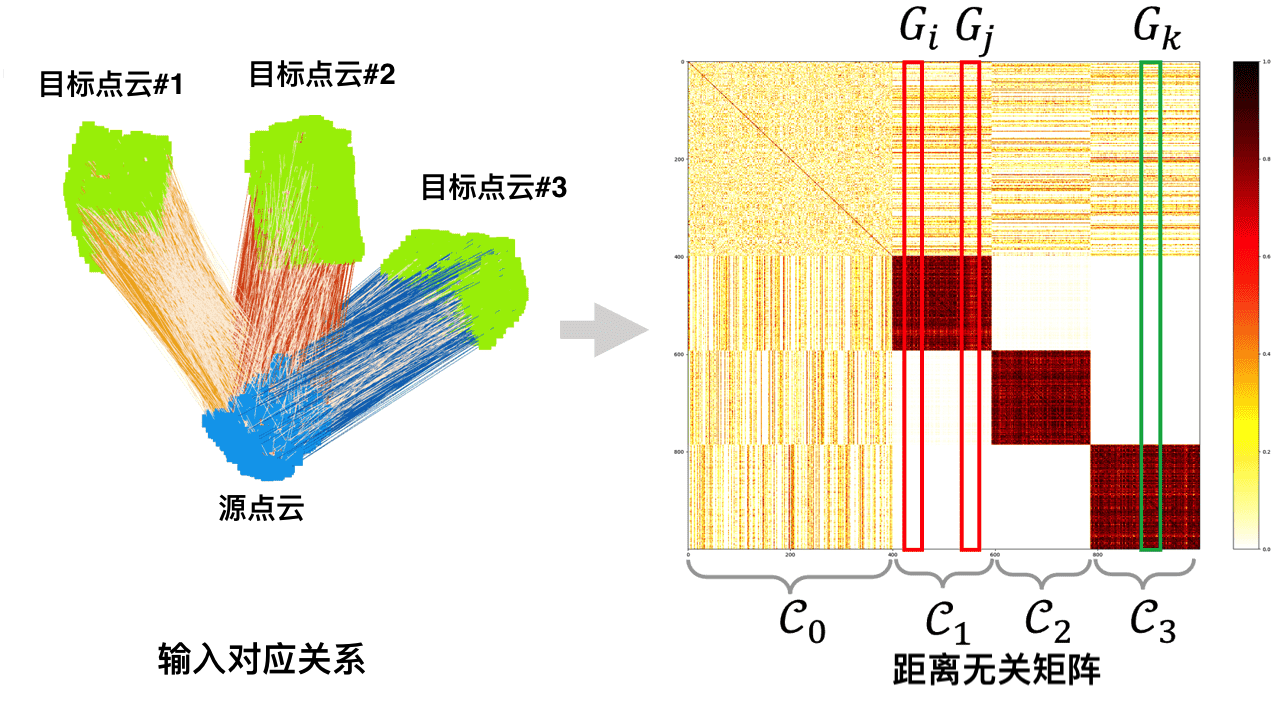
\includegraphics[width=0.7\textwidth]{images/matrix1.png} % 减小图像尺寸,使其略小于列宽。不要使用精确的图像宽度值。这样的设置可以避免过宽的盒子。
    \caption{距离不变性矩阵中的列向量(\emph{兼容性向量})包含了与实例相关的丰富信息。这里 $G_i,G_j$ 分别表示第 $i^{th}$ 和第 $j^{th}$ 对应关系的兼容性向量,它们都属于实例 $\mathcal{C}_1$。我们观察到 $G_i$ 与 $G_j$ 相似。相比之下,$G_i$ 与 $G_k$ 差异显著,因为第 $k^{th}$ 对应关系位于不同的实例 $\mathcal{C}_3$ 中。这里 $\mathcal{C}_0$ 代表异常值集合。请参阅第\ref{subsec:Distance-Consistency-Graph}节以获取详细信息。}
    \label{fig:matrix}
    \vspace{-0.6in}
\end{figure}

对应关系的兼容性向量可以被视为该对应关系的特征表示或“特征”。属于同一刚性变换的对应关系具有相似的特征。因此,基于这些兼容性向量,我们可以将对应关系聚类为与来自不同实例的内点相关的不同组。

\section{快速对应关系聚类}
我们以自底向上的方式聚类对应关系,这比现有方法采用的谱聚类\cite{parra2019practical}\cite{shi2021robin}要快得多。一开始,每个对应关系被视为一个独立的组。然后,我们反复合并距离最小的两个组,直到两个组之间的最小距离大于给定值($min_dist_thresh$)。定义组之间距离的方式产生了不同风格的算法。我们遵循\cite{Tlinkage}来定义距离。设$\mathbf{p}_i, \mathbf{p}_j$为两个组$i$和$j$的表示向量,组距离定义为
\begin{equation}
d(\mathbf{p}_i, \mathbf{p}_j)= 1-\frac{\langle \mathbf{p}_i,\mathbf{p}_j\rangle}{\parallel \mathbf{p}_i\parallel ^2+\parallel \mathbf{p}_j\parallel ^2-\langle \mathbf{p}_i,\mathbf{p}_j\rangle}.
\end{equation}
如果两个组合并,新组的表示向量更新为
$\mathbf{p}_i \leftarrow \min (\mathbf{p}_i, \mathbf{p}_j),$ 其中 $\min(\cdot)$ 表示取两个向量每个维度的最小值。
在聚类开始时,一个组(只包含一个对应关系)的表示向量设置为该对应关系的兼容性向量。

\section{递归簇细化} \label{sec:cluster_refinement}
在凝聚聚类之后,我们通过重复以下步骤来进一步优化结果,直到没有变化发生。

步骤1. 从对应关系数量大于阈值 $\alpha$ 的簇中估计刚性变换。

步骤2. 合并相似的变换。这一步将在下一节中解释。

步骤3. 为每个对应关系重新分配簇标签。将每个对应关系分配给对齐误差最小的变换。如果在所有变换中最小的对齐误差大于 $inlier_thresh$,则将对应关系标记为异常值。

在迭代过程中,对应关系变得越来越集中,因此我们可以在步骤1中调整 $\alpha$ 以增加异常值拒绝的强度。我们在每次迭代中更新 $\alpha$ 的策略如下:
\begin{equation}
\alpha \leftarrow \min(\alpha _0\times \theta ^{n-1},\left[N/100 \right] ),
\label{eq:alpha}
\end{equation}
其中 $n$ 表示第 $n^{th}$ 次迭代,$N$ 是对应关系的数量,$\left[ \cdot \right]$ 是四舍五入运算。在我们的实验中,我们设置 $\alpha_0 = 3$ 和 $\theta = 3$。细化过程通常在我们的实验中在三次迭代内收敛,因此效率也非常高。

\section{合并重复变换}
有时来自不同簇的相似变换会生成,这意味着它们可能属于同一个实例。在这种情况下,我们需要合并它们。
给定两个估计的变换 $(\mathbf{R}1, \mathbf{t}1)$ 和 $(\mathbf{R}2, \mathbf{t}2)$,我们计算每个对应关系的对齐误差,即 $e{ki} = |\mathbf{y}{i}-(\mathbf{R}k \mathbf{x}{i} + \mathbf{t}k)|^2, (k = 1,2)$。接下来,我们设置 $p{ki} = 1$ 如果 $e{ki} < inlier_thresh$,否则 $p{ki}=0$。因此,我们为两个变换获得两个二进制集 $P_1, P_2$。合并两个变换的条件是
\begin{equation}
IOU = |P_1 \cap P_2|/|P_1 \cup P_2| \geq 80%.
\label{eq:iou}
\end{equation}
如果满足这个条件,我们将放弃一个异常值较多的变换($p_{ki} = 0$)。然后我们根据在所有变换中对齐误差最小的一个重新为每个对应关系分配簇标签。

\section{从簇中提取变换}

在聚类之后,我们需要从这些对应关系簇中提取刚性变换。由于我们不知道目标点云中真实实例的数量,因此我们需要自动选择那些内点簇。我们首先选择内点簇的元素数量大于阈值(在我们的实验中为 $10$)并从这些簇中估计变换。接下来,我们根据其内点数量按降序对变换进行排序。一个变换拥有的内点越多,它与真实实例相关联的可能性就越高。最后,我们检查内点数量在变换之间的降低比例,以及第一个变换(具有最多内点)之间的比例,通过
\begin{equation}
    \gamma_k = \#I_{k}/\#I_{0},\,\, k = 1,2,\ldots
\end{equation}

其中 $\#I_k$ 表示第 $k^{th}$ 变换的内点数量。如果 $\gamma_k <= \gamma_thresh$,我们忽略所有在 $k$ 之后的变换。$\gamma_thresh$ 可以更改以在召回和精确度之间进行权衡。

\section{处理大量对应关系}
% TODO down_sample and cluster
% 1.unsample
% 为什么要downsample,downsample为什么可行
当输入对应关系的数量很大时,计算距离不变矩阵和聚类对应关系可能会变得昂贵。我们通过添加下采样和上采样过程来解决这个问题。在构建距离不变矩阵之前进行下采样过程,通过随机抽样固定数量的对应关系(在我们的实现中为 $1024$)进行进一步处理。在选定对应关系聚类之后进行上采样过程,将所有对应关系分配给现有簇。分配是通过选择对齐误差最小的变换来完成的,如第 \ref{sec:cluster_refinement} 节中的步骤3所述。
%%
% The BIThesis Template for Bachelor Paper Translation
%
% 北京理工大学毕业设计(论文) —— 使用 XeLaTeX 编译
%
% Copyright 2020-2023 BITNP
%
% This work may be distributed and/or modified under the
% conditions of the LaTeX Project Public License, either version 1.3
% of this license or (at your option) any later version.
% The latest version of this license is in
%   http://www.latex-project.org/lppl.txt
% and version 1.3 or later is part of all distributions of LaTeX
% version 2005/12/01 or later.
%
% This work has the LPPL maintenance status `maintained'.
%
% The Current Maintainer of this work is Feng Kaiyu.
%
% Compile with: xelatex -> biber -> xelatex -> xelatex
%%

% 第一章节

\chapter{实验验证}


我们在合成数据集和真实世界数据集上进行实验,将我们的方法与三种最先进的多模型拟合方法进行比较:T-linkage(2014)\cite{Tlinkage},Progressive-X(2019)\cite{ProgressiveX} 和 CONSAC(2020)\cite{CONSAC}。其他多模型拟合方法:RPA\cite{RPA} 和 RansaCov\cite{Coverage} 非常慢(需要几个月的时间)来运行我们的实验,因此我们没有包括它们。我们还展示了最先进的一对一配准方法 TEASER(2020)\cite{TEASER} 的结果作为比较。我们仔细调整所有方法,在合理的时间和内存消耗范围内,在评估数据集上实现最佳性能。为了公平比较,所有方法都使用相同的点对应关系集作为输入。

我们使用 Pytorch\cite{Pytorch} 实现我们的算法。T-linkage 和 Progressive-X 是纯 CPU 算法,而 CONSAC 是基于 GPU 的学习方法。我们在与 T-linkage 和 Progressive-X 相同的 CPU(Intel Core i7-8700K)上运行我们的算法,并在与 CONSAC 相同的 GPU(GTX 1080Ti)上运行。我们的方法有三个参数,其中在我们的实验中设置为 $min\_dist\_thresh=0.2$, $inlier\_thresh=0.3$ and $\gamma\_thresh=0.5$。所有点云都在 $0.05m$ 体素大小中进行下采样。正如补充材料中的消融研究所示,我们的方法对参数变化不敏感。

由于一对一配准中使用的指标不能用于多实例设置,我们从检索任务中采用三个评估指标:MHR(Mean Hit Recall),MHP(Mean Hit Precision),MHF1(Mean Hit F1)。它们的定义详见补充材料。

    
\section{合成数据集}
我们从 PointNet++\cite{pointnet2} 预先采样的 Modelnet40 数据集\cite{ModelNet40} 生成一个合成数据集。
我们将每个点云下采样到 $256$ 个点,并随机生成 $K$ 个变换(在我们的测试中最多为 $20$),形成一个目标点云。目标点云还与其他对象和随机点混合,以更好地模拟真实世界情况。
    
\begin{figure*}[ht]
    \centering
    \begin{subfigure}{0.4\textwidth}
        \centering
        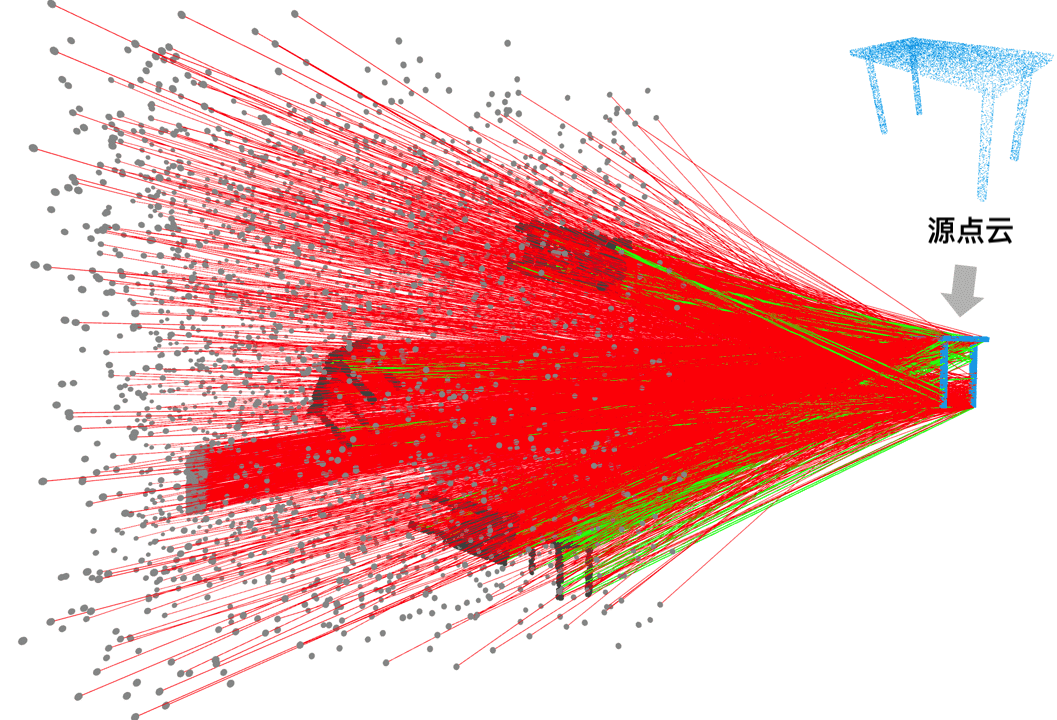
\includegraphics[height=3cm]{images/multi-input-corrs.png}
          \caption{输入匹配关系(离群点比重 : $95.5\%$) }
          \label{fig:multi-corrs}
      \end{subfigure}
      \begin{subfigure}{0.45\textwidth}
        \centering
        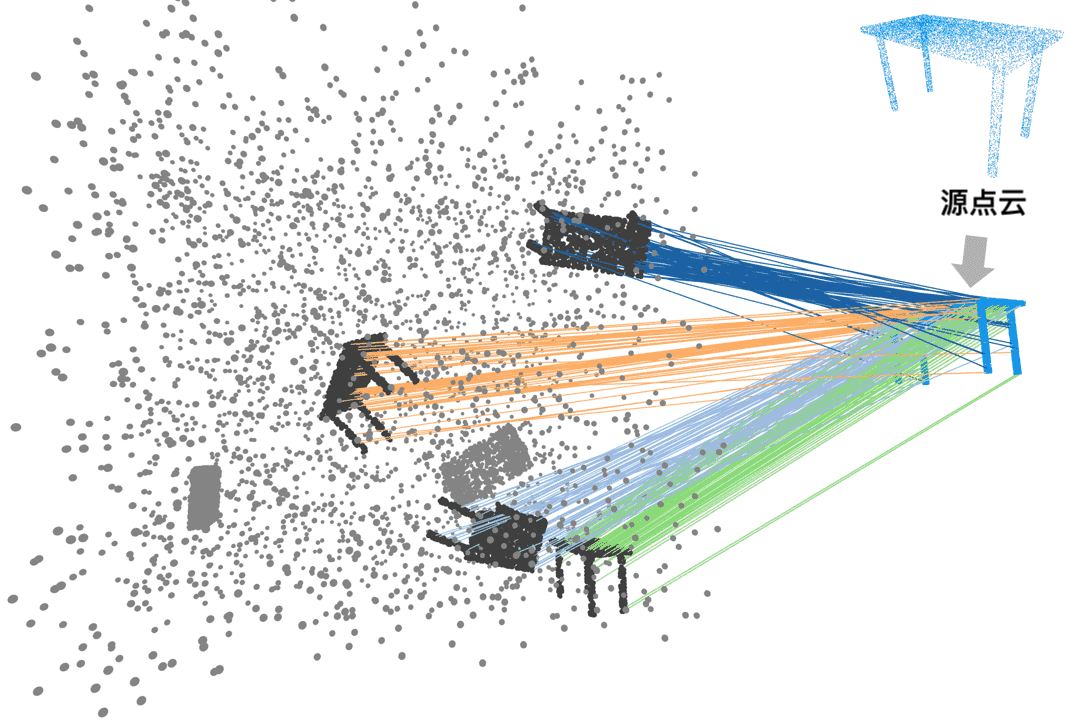
\includegraphics[height=3cm]{images/multi-cluster-corrs.png}
          \caption{我们的聚类结果}
          \label{fig:multi-cluster-corrs}
      \end{subfigure}
  
  
      \begin{subfigure}{0.18\textwidth}
        \centering
        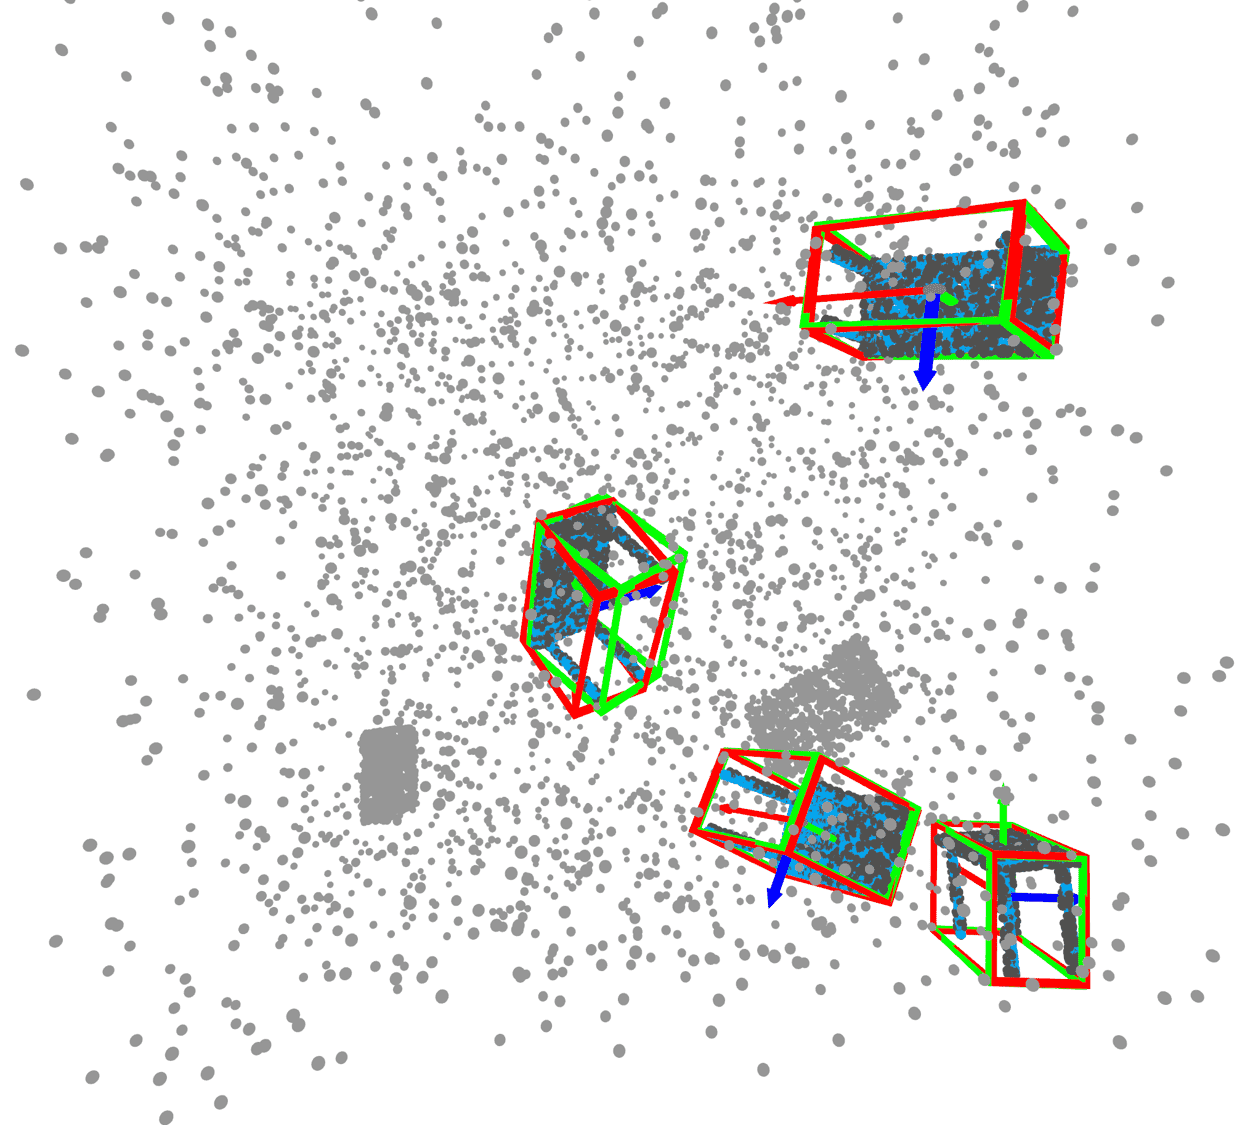
\includegraphics[height=2.8cm]{images/multi-ours.png}
          \caption{Ours}
          \label{fig:multi-result}
      \end{subfigure}
      \begin{subfigure}{0.18\textwidth}
        \centering
        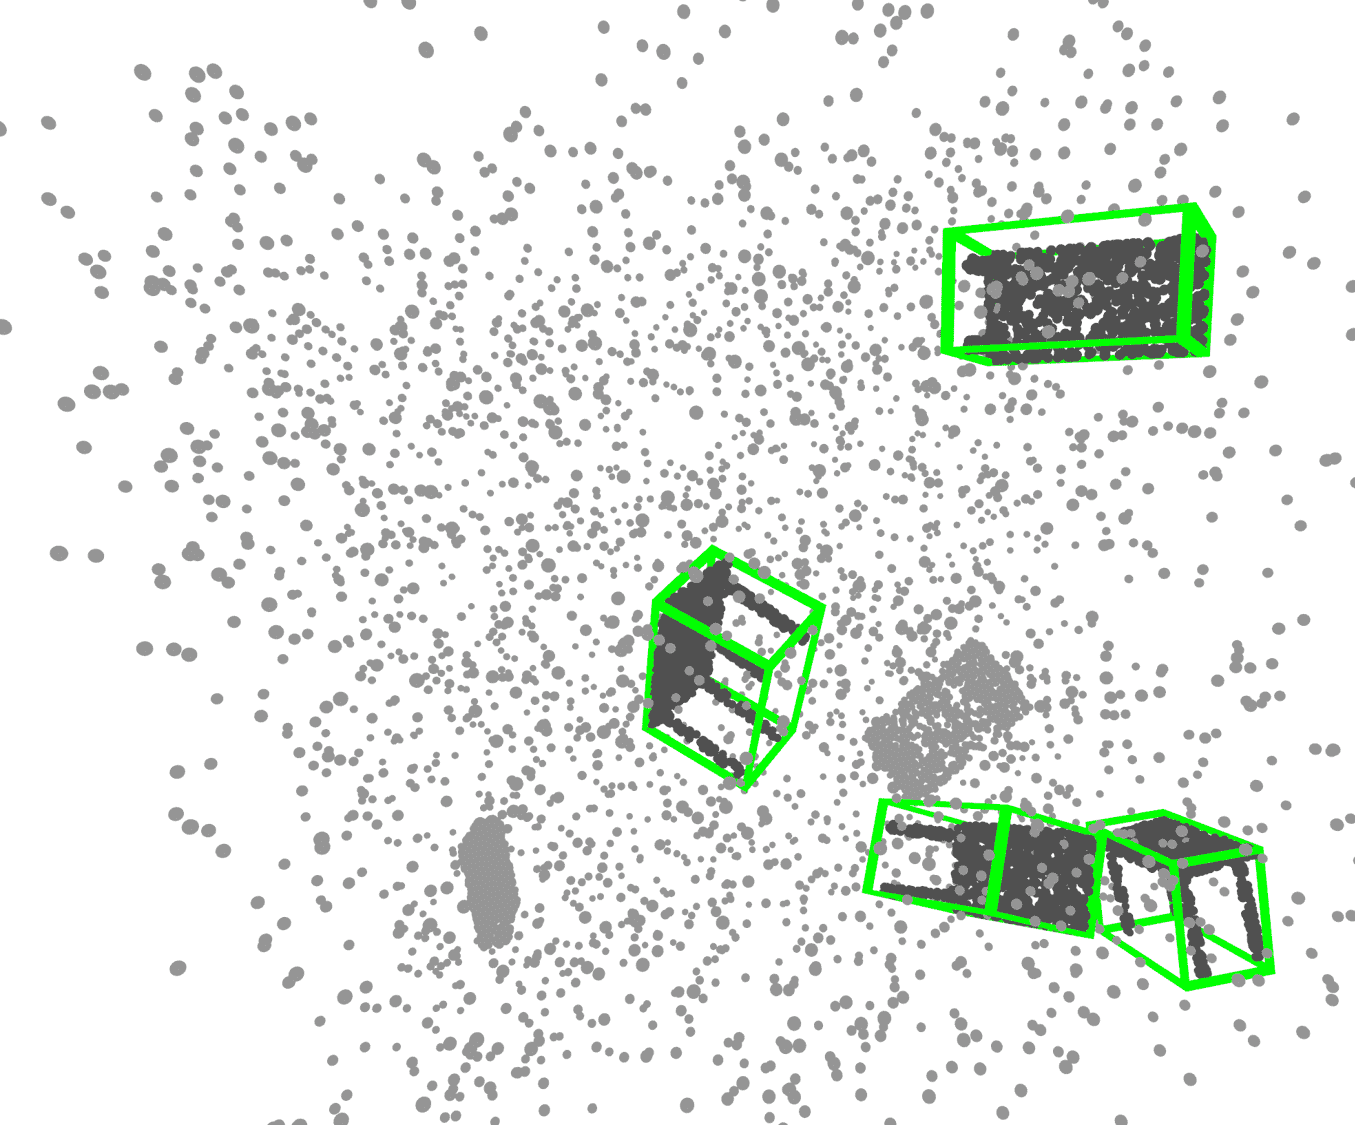
\includegraphics[height=2.8cm]{images/multi-tlinkage.png}
          \caption{T-Linkage\cite{Tlinkage}}
          \label{fig:multi-tlinkage1}
      \end{subfigure}
      \begin{subfigure}{0.2\textwidth}
        \centering
        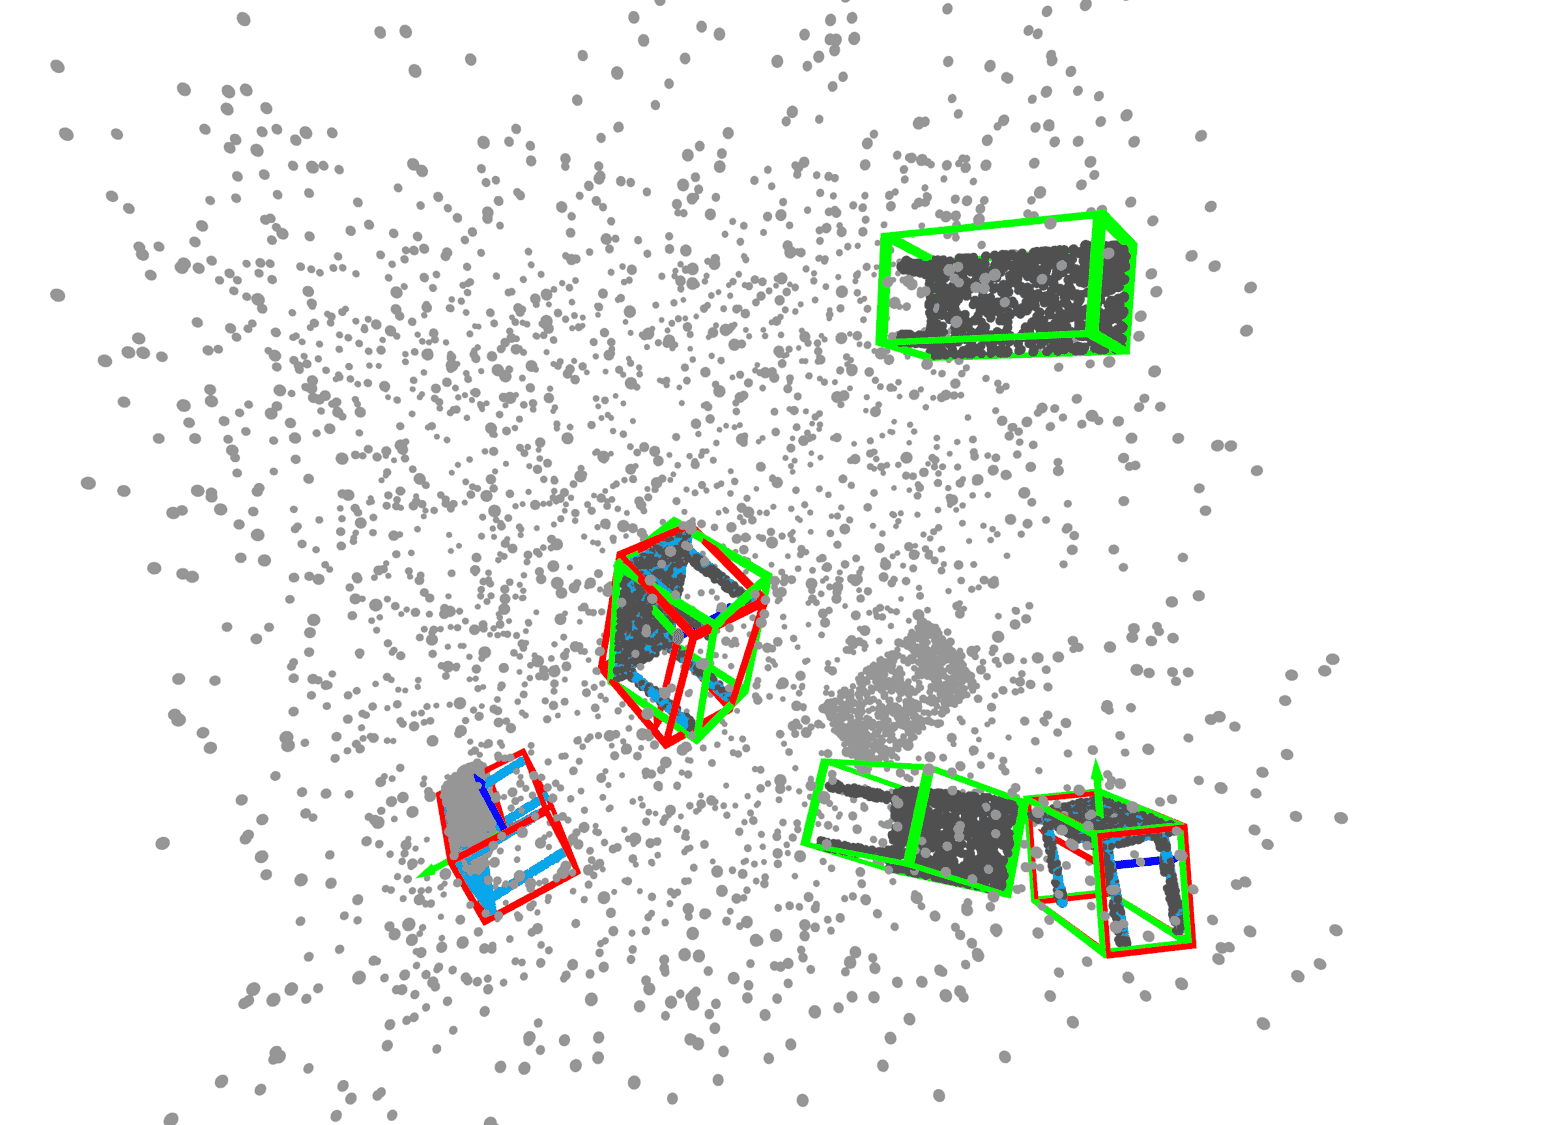
\includegraphics[height=2.8cm]{images/multi-progx.png}
          \caption{Progressive-X\cite{ProgressiveX}}
          \label{fig:multi-prox}
      \end{subfigure}
      \begin{subfigure}{0.2\textwidth}
        \centering
        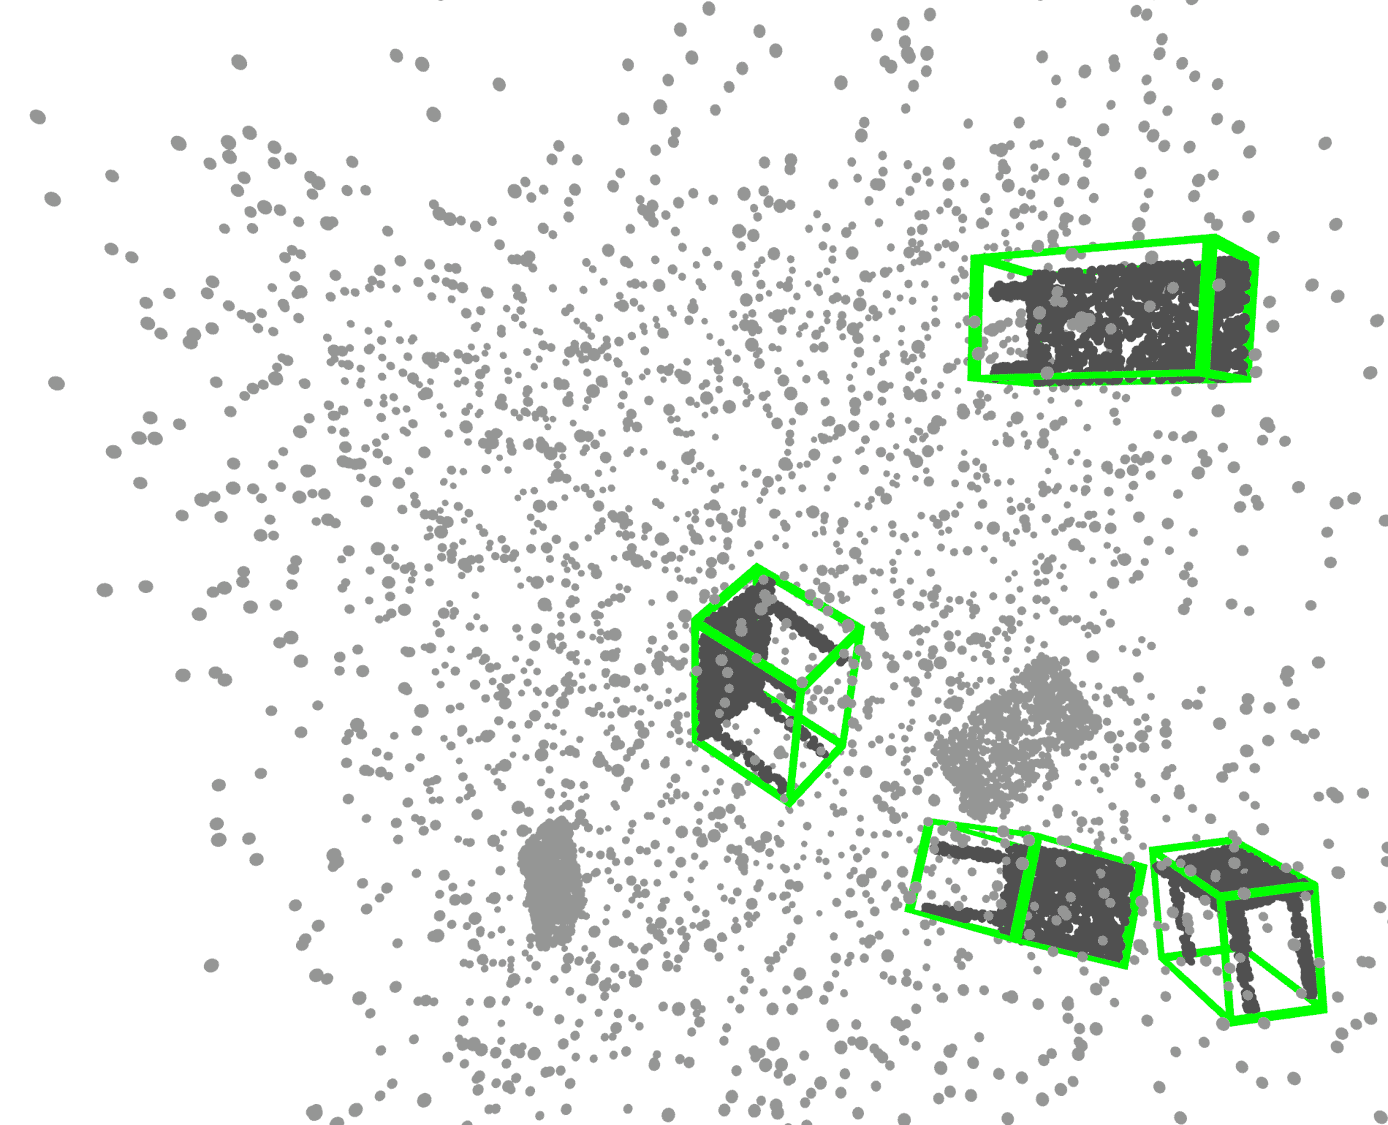
\includegraphics[height=2.8cm]{images/multi-consac.png}
          \caption{CONSAC\cite{CONSAC}}
          \label{fig:multi-consac}
      \end{subfigure}
      \begin{subfigure}{0.18\textwidth}
        \centering
        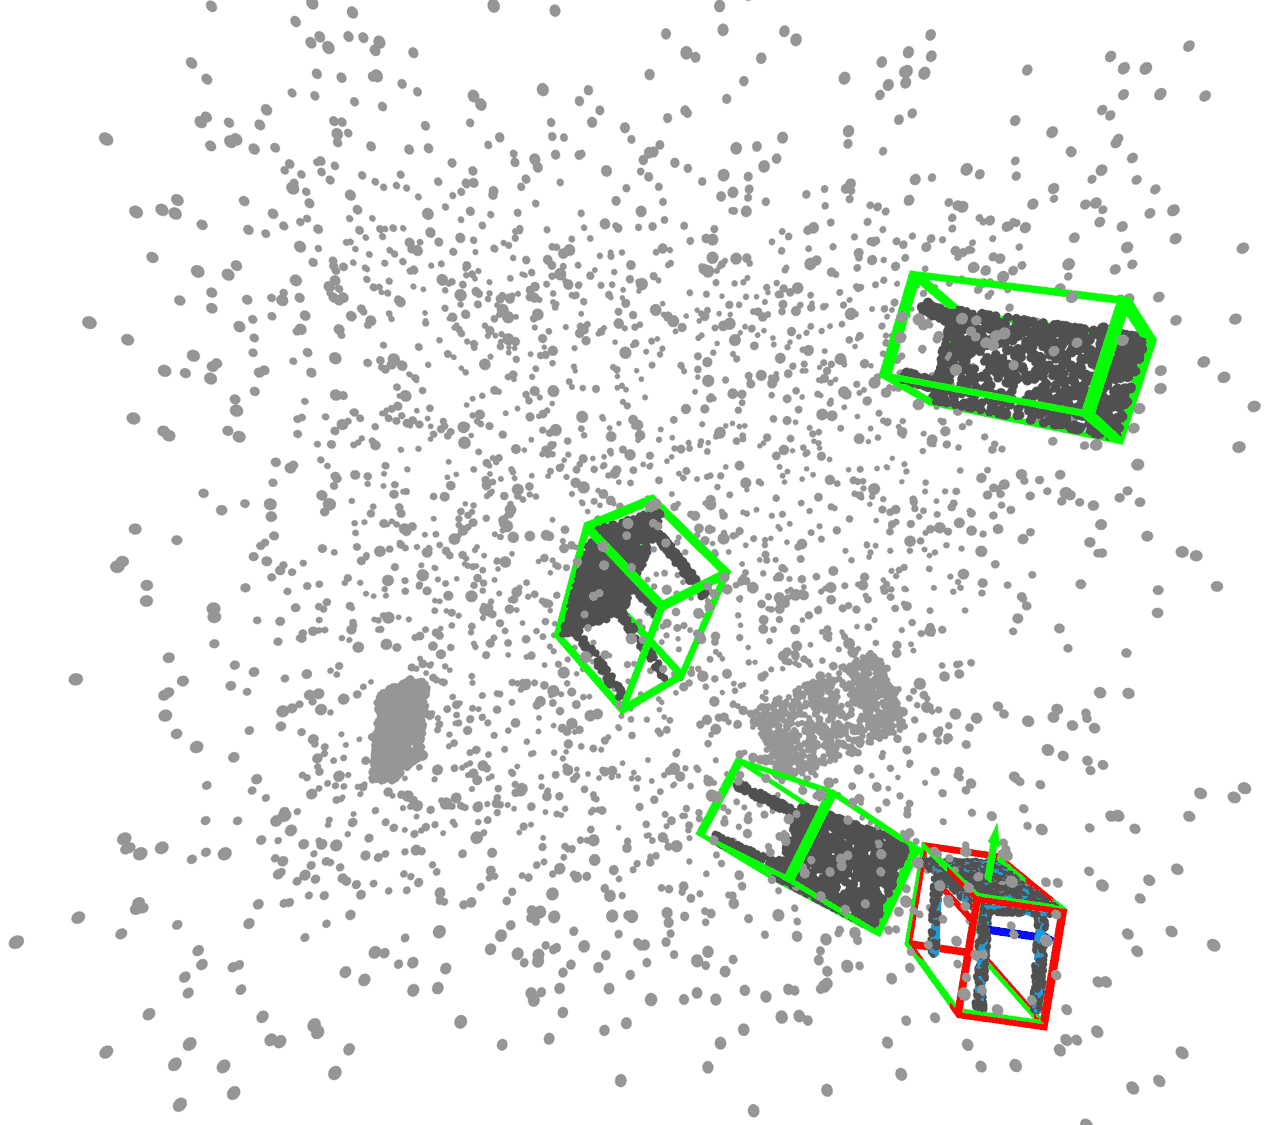
\includegraphics[height=2.8cm]{images/multi-teaser.png}
          \caption{TEASER\cite{TEASER}}
          \label{fig:multi-teaser}
      \end{subfigure}
      % \begin{subfigure}{0.18\textwidth}
      %   \centering
      %   \includegraphics[height=2.5cm]{scan2cad-cad-ransac1.png}
      %     \caption{RANSAC}
      %     \label{fig:scan2cad_cad-ransac1}
      % \end{subfigure}
  
  %\includegraphics[width=0.9\columnwidth]{figure/} % Reduce the figure size so that it is slightly narrower than the column. Don't use precise values for figure width.This setup will avoid overfull boxes.
  \caption{\textbf{在数据集上的结果。} (a) 通过匹配 PREDATOR\cite{PREDATOR} 特征得到的输入对应关系。内点和离群点分别用绿色和红色显示。 (b) 我们的聚类结果用不同的颜色显示(只显示内点)。在 (c-g) 中,我们用红色框显示估计的位姿,用绿色框显示真实位姿。我们的方法 (c) 配准了所有实例。T-linkage (d) 和 CONSAC (f) 无法配准任何实例。Progressive-X (e) 配准了 2 个实例,但产生了错误的配准。TEASER (g) 配准了一个实例。}
  \label{fig:predatormm}
  \end{figure*}
    
\paragraph{仿真对应关系}
在这个测试中,我们直接通过混合地面真实值和离群值来生成输入对应关系。我们测试了不同的离群比例,$10\%\sim50\%$,$50\%\sim70\%$ 和 $70\%\sim90\%$。请注意,对于每个测试样本,离群点是在给定范围内随机抽样的。结果显示在表 \ref{tab:mm} 中。随着离群比例的增加,几乎所有方法的性能都有所下降,但我们的方法下降缓慢,且仍然明显优于其他方法。我们的算法在 CPU 或 GPU 上的速度比现有方法快 10 倍。
我们还在图 \ref{fig:detail-mm}(a) 中绘制了我们的方法在不同离群比例下的 MHF1(Mean Hit F1) 曲线,其中包括 $20$ 个实例。尽管当离群比例非常大时性能迅速下降,但我们的方法在 $70\%$ 的离群比例下仍然能达到 $90.46\%$ 的 MHF1。图 \ref{fig:detail-mm}(b) 显示了在固定离群比例 $50\%$ 的情况下,不同实例数量的 MHF1 曲线。即使存在 $30$ 个实例,我们的方法的 MHF1 也约为 $92.73\%$。
  

\begin{table}[ht]
    \centering
\scriptsize
    %\resizebox{.95\columnwidth}{!}{
    \begin{tabular}{ccccc} %& $50\%~70\%$ & $70\%~90\%$
        \toprule
        % & MHR$\left( \% \right) \uparrow $ & MRRE $\left( \right) \downarrow $ & MRTE & Time\\
        \textbf{方法}& MHR$\left( \% \right) \uparrow $ & MHP$\left( \% \right) \uparrow $ & MHF1$\left( \% \right) \uparrow $ & 时间$\left( s \right) \downarrow $\\
        \hline
        \multicolumn{5}{c}{离群点比重 : $10\%\sim50\%$} \\
        \hline
        T-Linkage & 3.05 & 14.80 & 4.65& 57.27 \\
        Progressive-X & 27.91 & 80.28 & 41.04 & 87.25\\
        CONSAC & 0.47 & 0.47 & 0.47 & 9.23  \\
        \textbf{Ours} & \textbf{96.08} & \textbf{99.73} & \textbf{97.03} & \textbf{0.62/0.30} \\ % 前gt_num个预测值的recall
        \hline
        \multicolumn{5}{c}{离群点比重 : $50\%\sim70\%$} \\
        \hline
        %\hline
        % \textbf{metric} & MHR$\left( \% \right) \uparrow $ & RRE$\left( \degree \right) \downarrow $ & RTE$\left( m \right) \downarrow $ & t$\left( s \right) \downarrow $\\
        %\hline
        %\hline
        T-Linkage & 1.33 & 7.00 & 2.05 & 56.90 \\
        Progressive-X & 20.60 & 75.10 & 31.70 & 85.54  \\
        CONSAC & 0.49 & 0.49 & 0.49 & 9.55\\
        \textbf{Ours} & \textbf{93.99} & \textbf{99.49} & \textbf{95.51} & \textbf{0.55/0.28}\\
        \hline
        
        \multicolumn{5}{c}{Outlier ratio : $70\%\sim90\%$} \\
        \hline
        %\hline
        % \textbf{metric} & MHR$\left( \% \right) \uparrow $ & RRE$\left( \degree \right) \downarrow $ & RTE$\left( m \right) \downarrow $ & t$\left( s \right) \downarrow $\\
        %\hline
        %\hline
        T-Linkage & 0.81 & 4.42 & 1.25 & 56.89 \\
        Progressive-X & 12.88 & 62.60 & 20.73 & 84.5 \\
        CONSAC & 0.51 & 0.51 & 0.51 & 7.70  \\
        \textbf{Ours} & \textbf{60.39} & \textbf{94.42} & \textbf{69.36} &\textbf{0.50/0.24}\\

        \hline
        \multicolumn{5}{c}{离群点比重 : $90\%\sim99\%$} \\
        \hline
        T-Linkage & 0.28 & 1.30 & 0.42 & 56.69 \\
        Progressive-X & 7.13 & 39.19 & 11.67 & 84.43\\
        CONSAC & 0.51 & 0.51 & 0.51 & 9.57  \\
        \textbf{Ours} & \textbf{14.70} & \textbf{65.20} & \textbf{22.75} & \textbf{0.47/0.21} \\ % 前gt_num个预测值的recall
        \bottomrule
        %outlier ratio & $10\%~50\%$ & $50\%~70\%$ & $70\%~90\%$\\

    \end{tabular}
    \caption{在不同离群比例的合成对应关系上的结果。$\uparrow$ 表示越大越好,而 $\downarrow$ 表示相反。我们方法在 CPU/GPU 上的运行时间也展示出来。}
    \label{tab:mm}
    \end{table}
    
\begin{figure}[ht]
    \centering
    \begin{subfigure}{0.4\textwidth}
        \centering   
        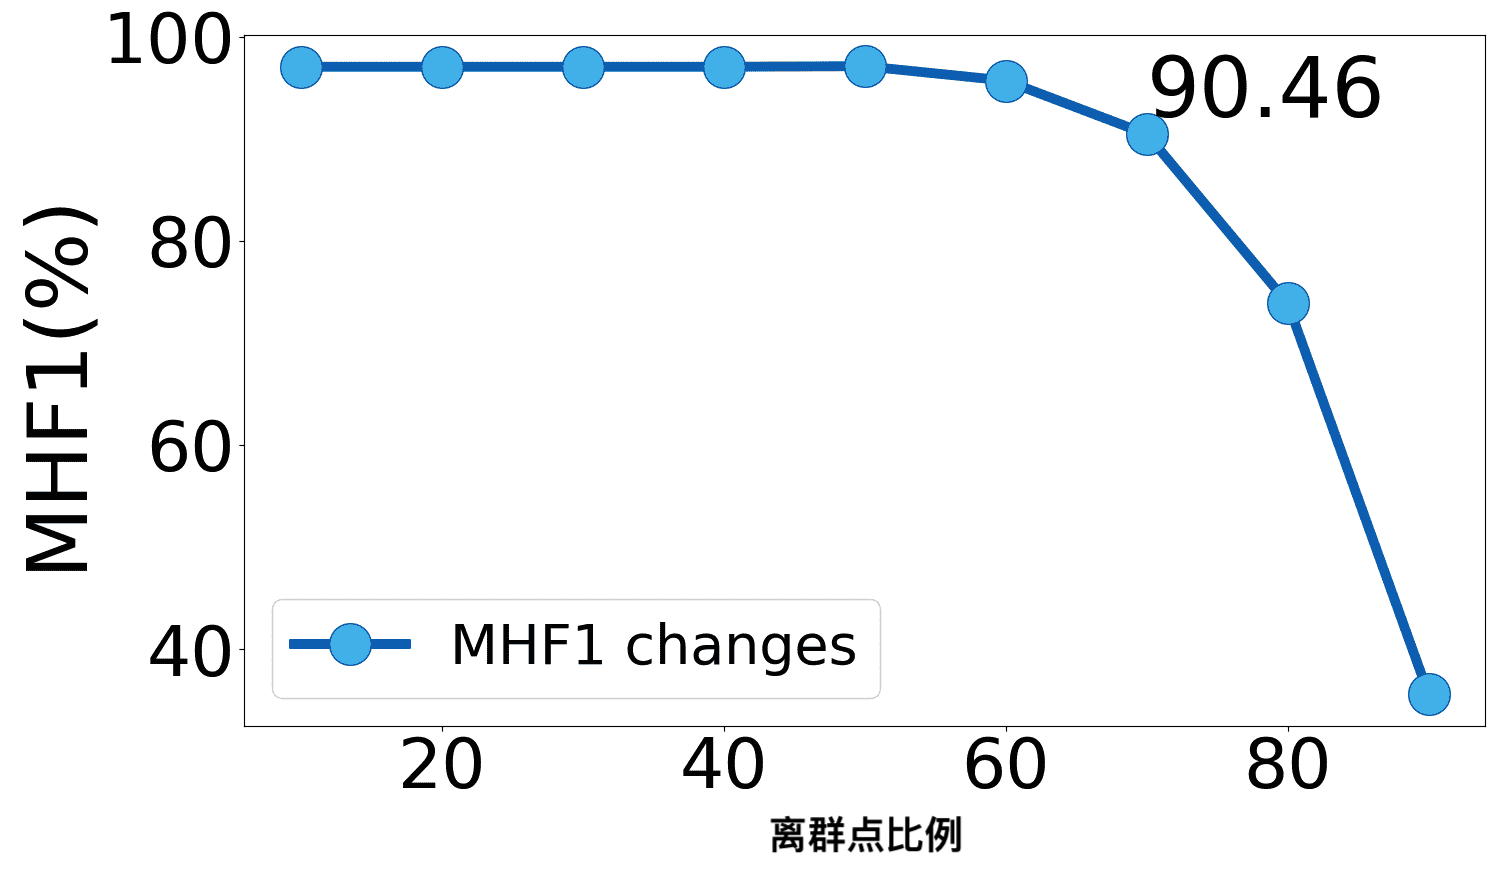
\includegraphics[width=\linewidth]{images/mhf1_or.png}
          \caption{}
      \end{subfigure}
      \begin{subfigure}{0.4\textwidth}
        \centering   
        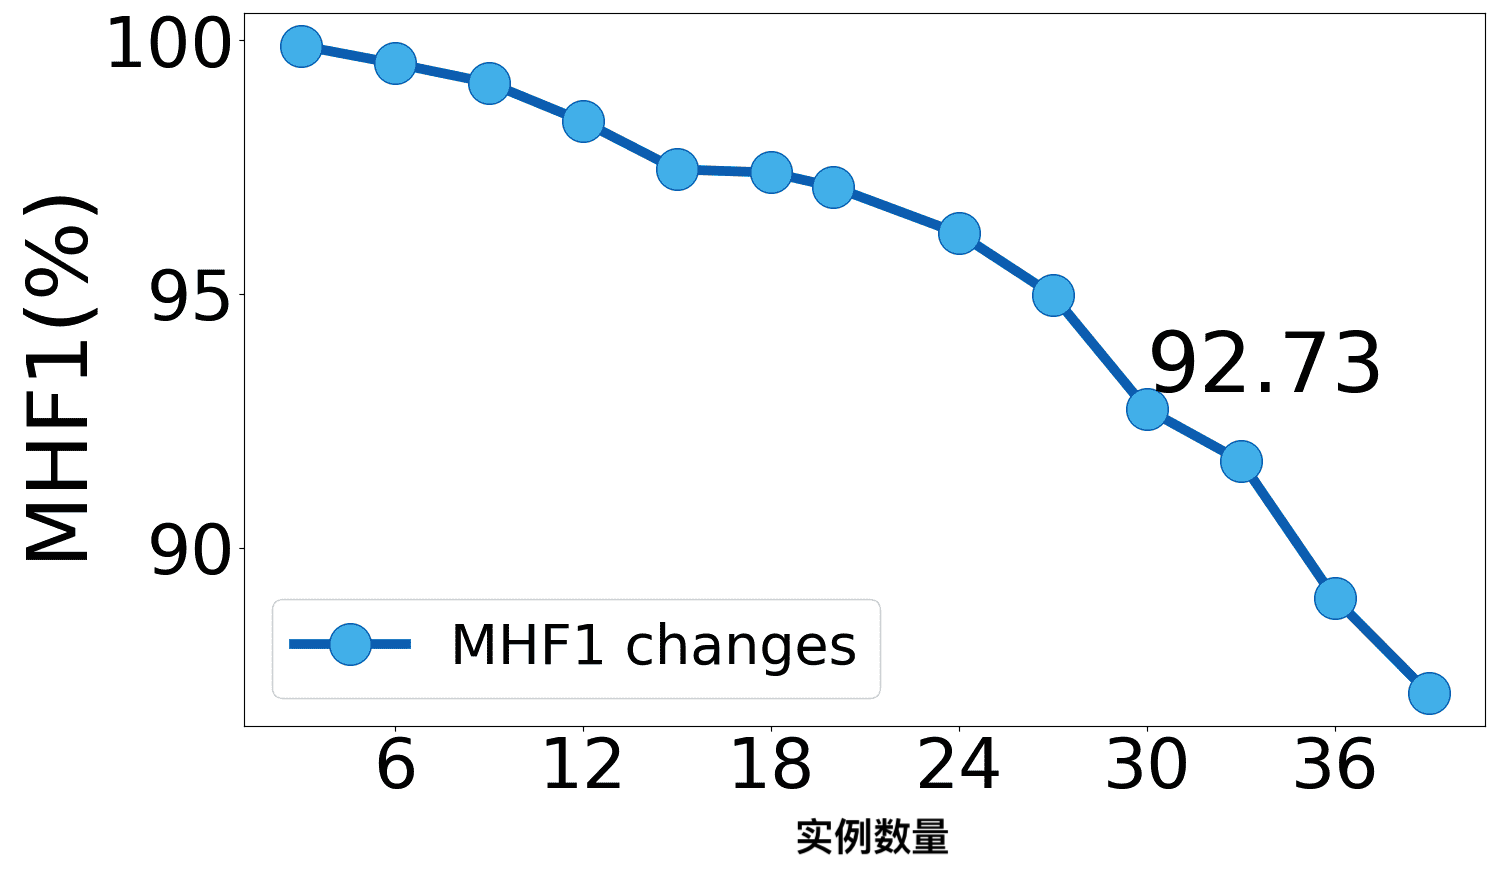
\includegraphics[width=\linewidth]{images/mhf1_in.png}
          \caption{}
          \label{fig:multi-instance}
      \end{subfigure} % Reduce the figure size so that it is slightly narrower than the column. Don't use precise values for figure width.This setup will avoid overfull boxes.
    \caption{(a) 平均 Hit F1 与离群比例关系。 (b) 平均 Hit F1 与实例数量关系(固定离群比例为 $50\%$)。}
    \label{fig:detail-mm}
    %\label{fig:multi-instance}
\end{figure}

\begin{figure*}[ht]
    \centering
    \begin{subfigure}{0.41\textwidth}
        \centering
        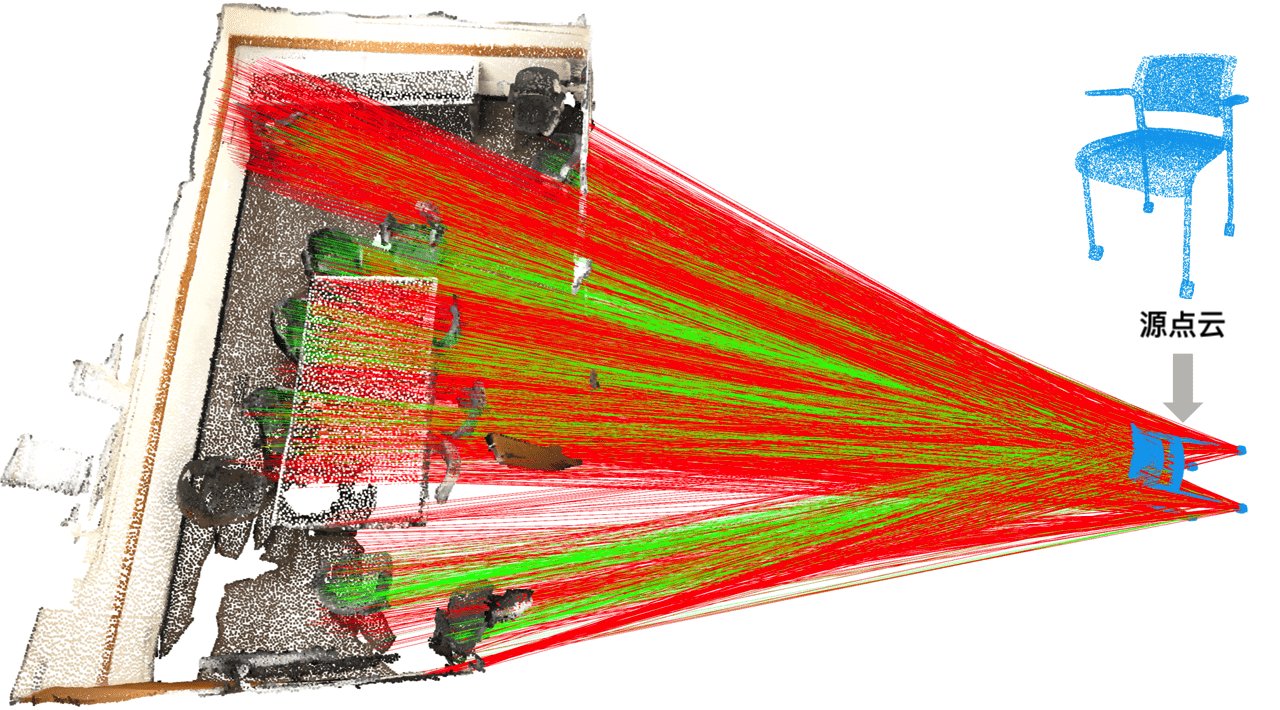
\includegraphics[height=2.8cm]{images/scan2cad-cad-input-corrs.png}
          \caption{Input correspondences}
          \label{fig:scan2cad_cad-input-corrs}
      \end{subfigure}
      \begin{subfigure}{0.41\textwidth}
        \centering
        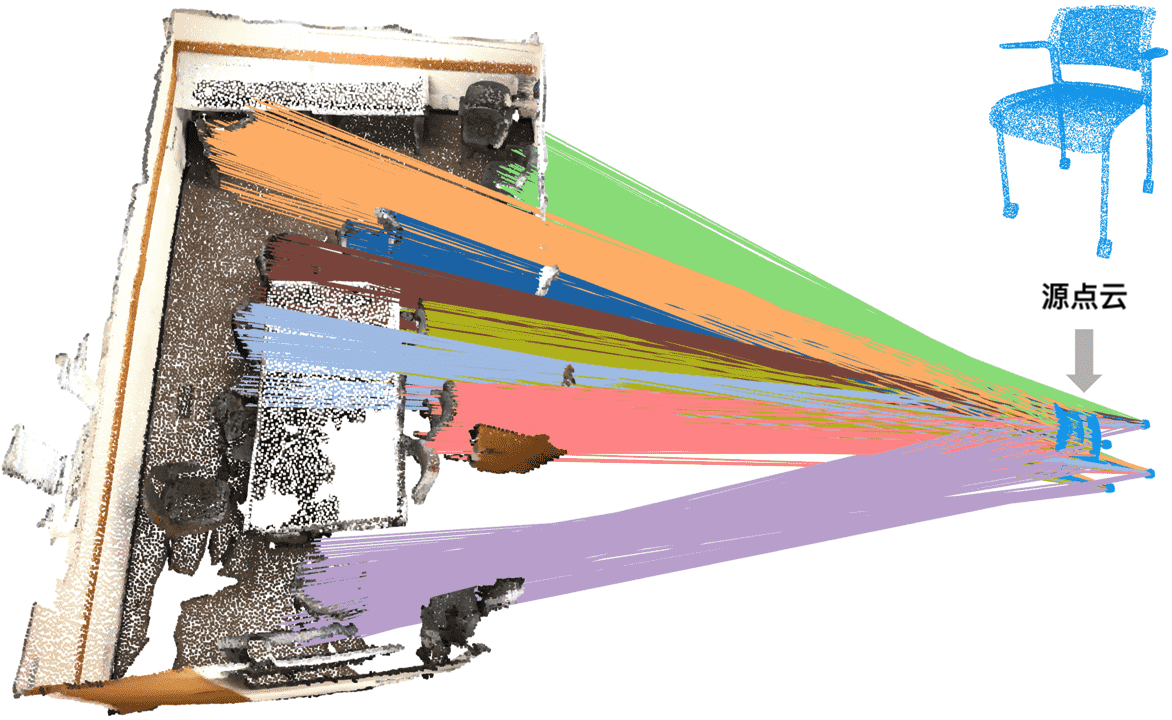
\includegraphics[height=2.8cm]{images/scan2cad-cad-cluster-corrs.png}
          \caption{Our clustering result}
          \label{fig:scan2cad_cad-cluster-corrs}
      \end{subfigure}

      
      \begin{subfigure}{0.18\textwidth}
        \centering
        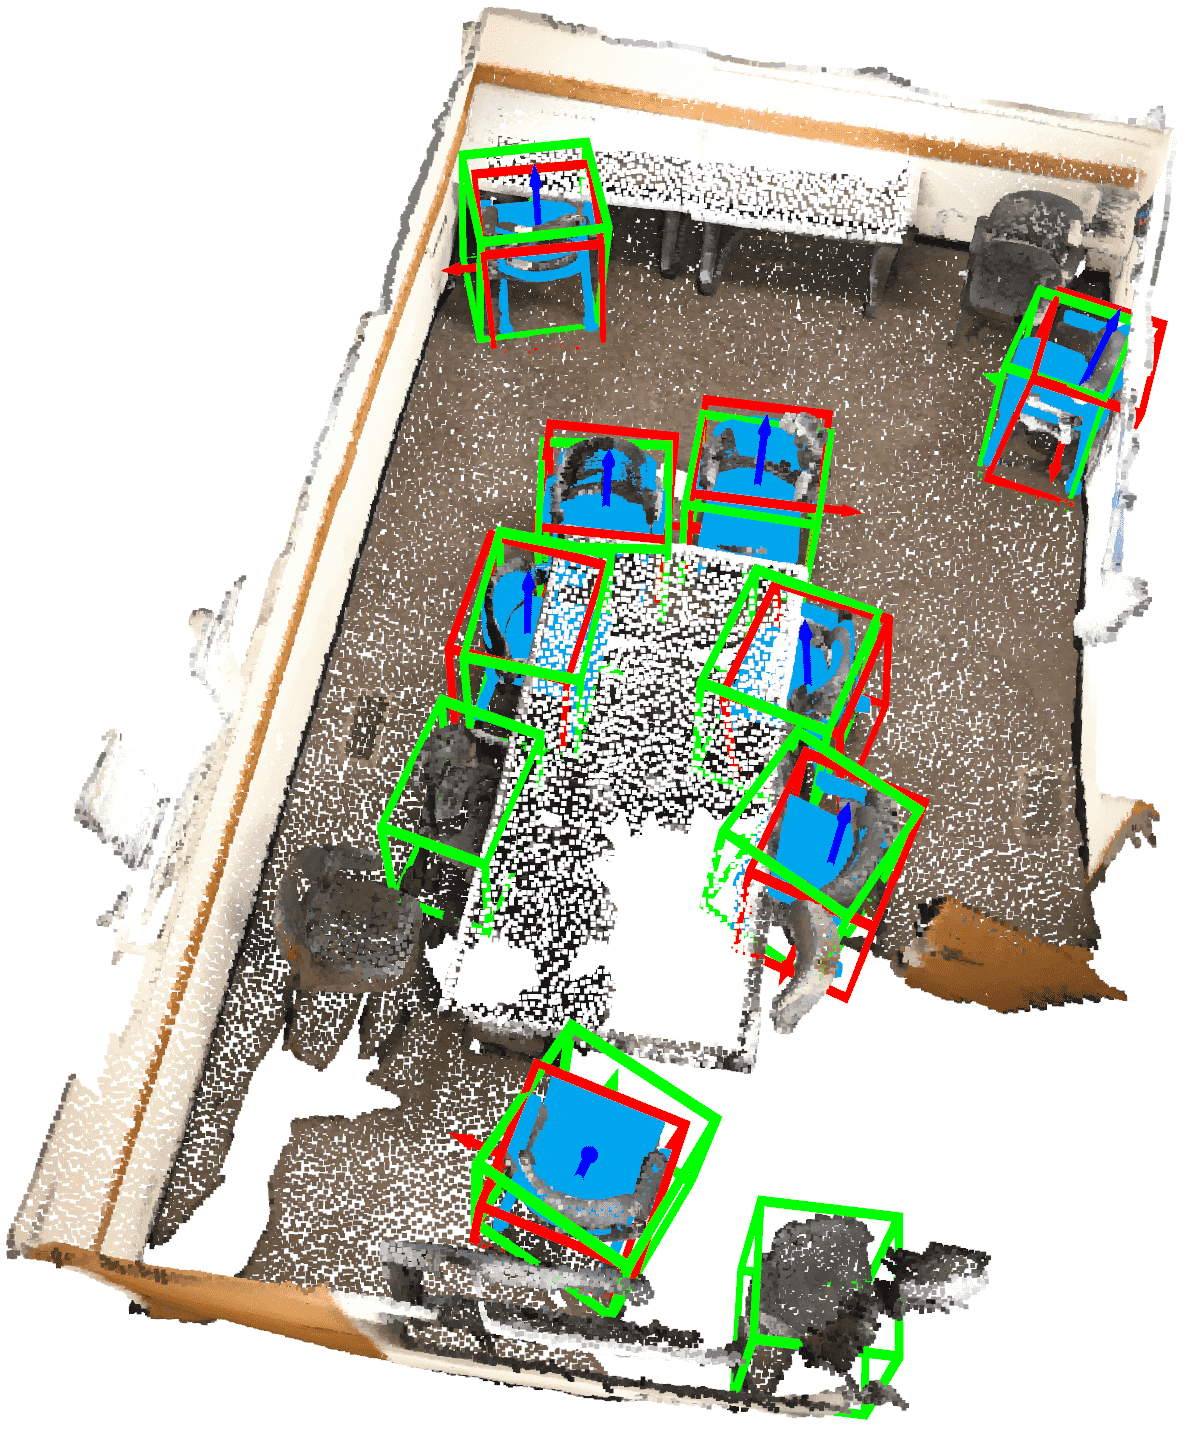
\includegraphics[height=3.3cm]{images/scan2cad-cad-ours.png}
          \caption{Ours}
          \label{fig:scan2cad_cad-result}
      \end{subfigure}
      \begin{subfigure}{0.18\textwidth}
        \centering
        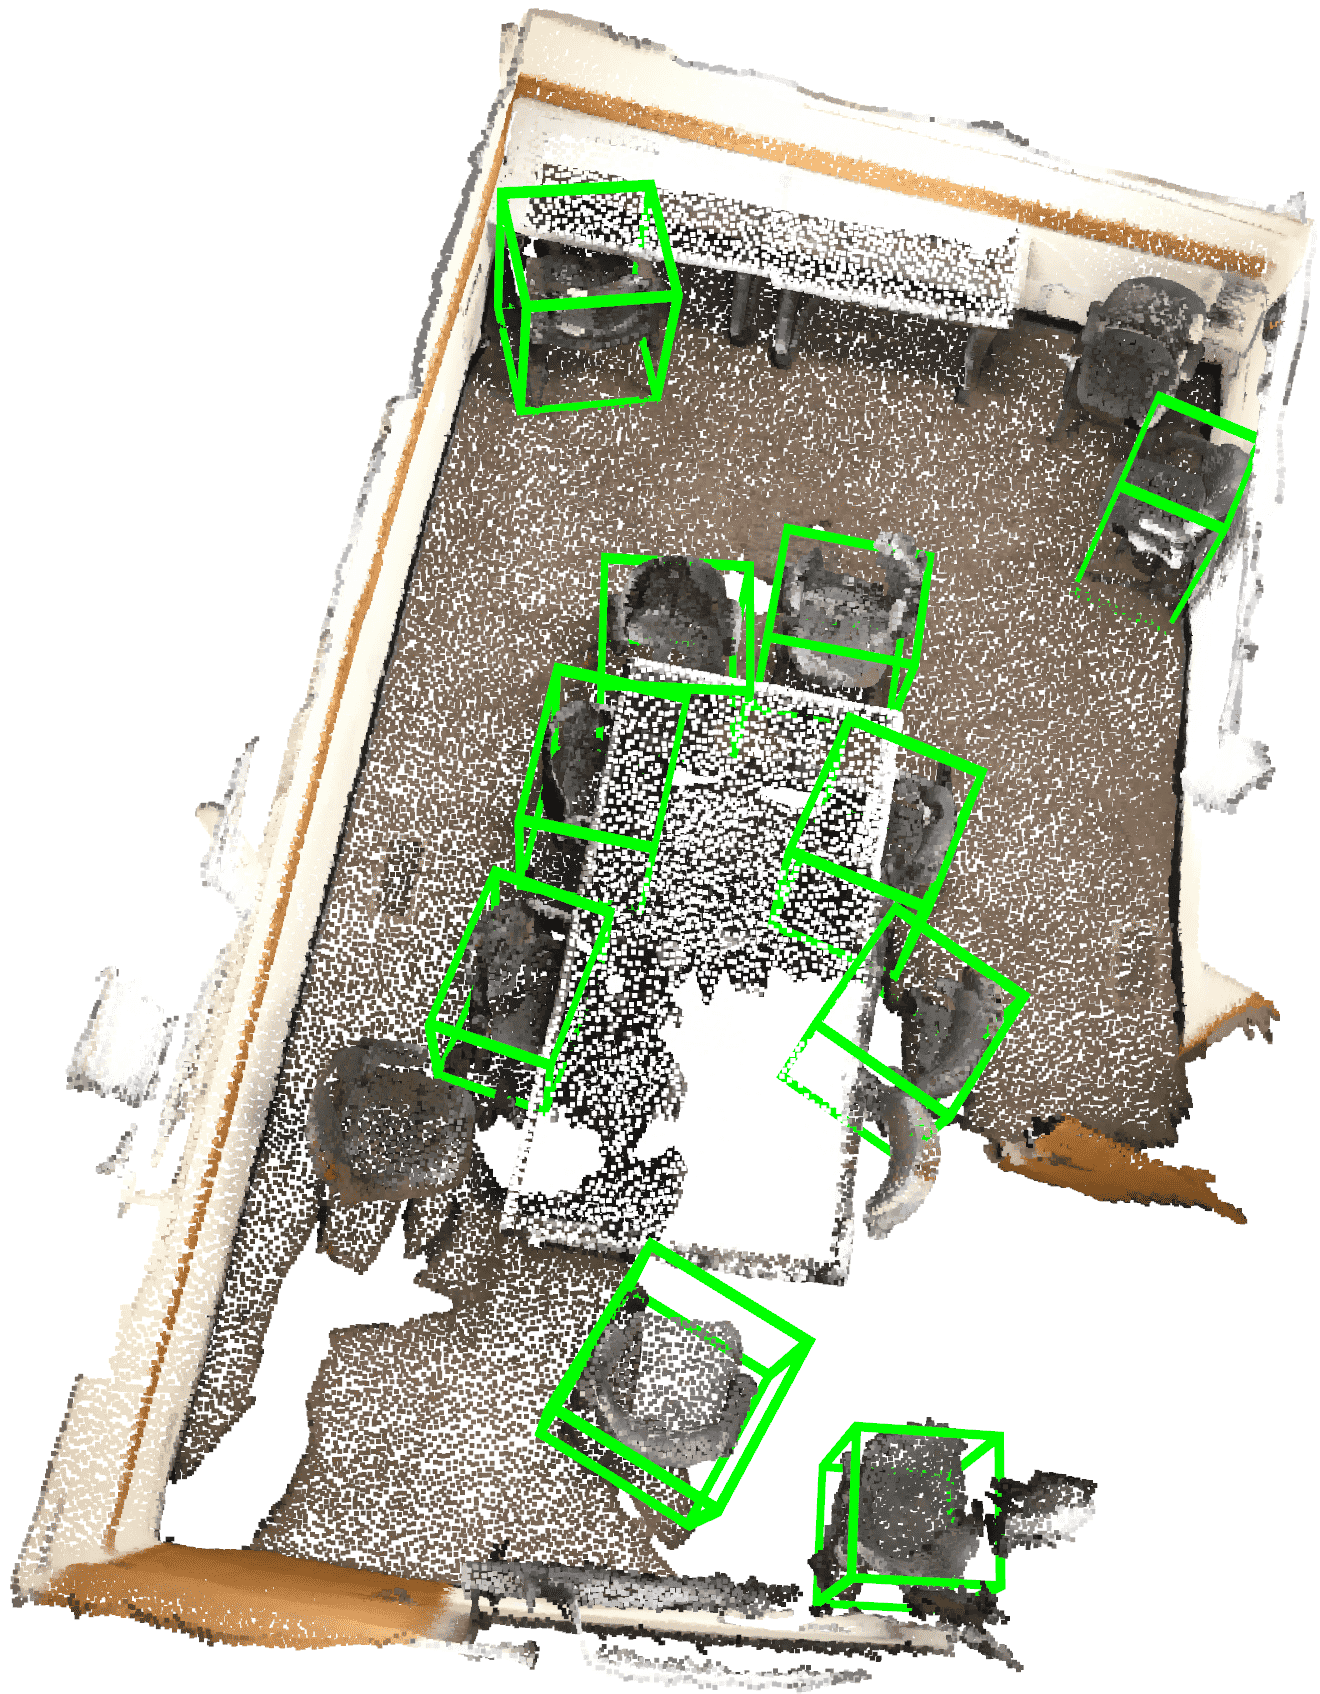
\includegraphics[height=3.3cm]{images/scan2cad-cad-tlinkage.png}
          \caption{T-linkage\cite{Tlinkage}}
          \label{fig:scan2cad_cad-tlinkage}
      \end{subfigure}
      \begin{subfigure}{0.19\textwidth}
        \centering
        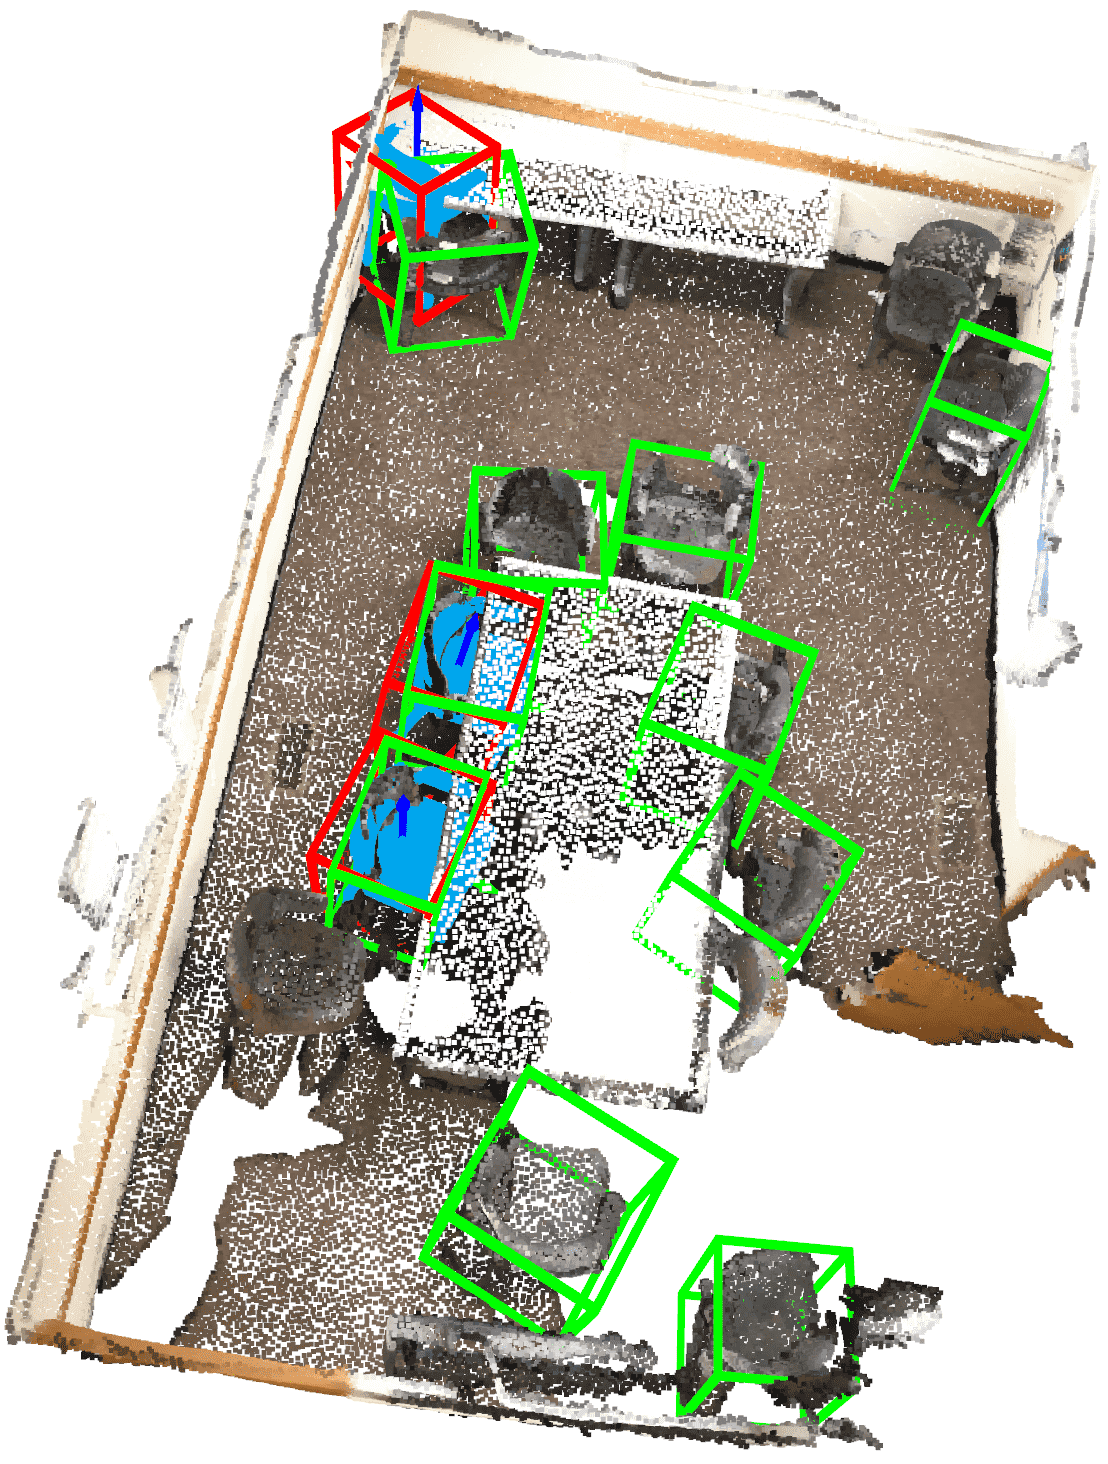
\includegraphics[height=3.3cm]{images/scan2cad-cad-progx.png}
          \caption{Progressive-X\cite{ProgressiveX}}
          \label{fig:scan2cad_cad-prox}
      \end{subfigure}
      \begin{subfigure}{0.17\textwidth}
        \centering
        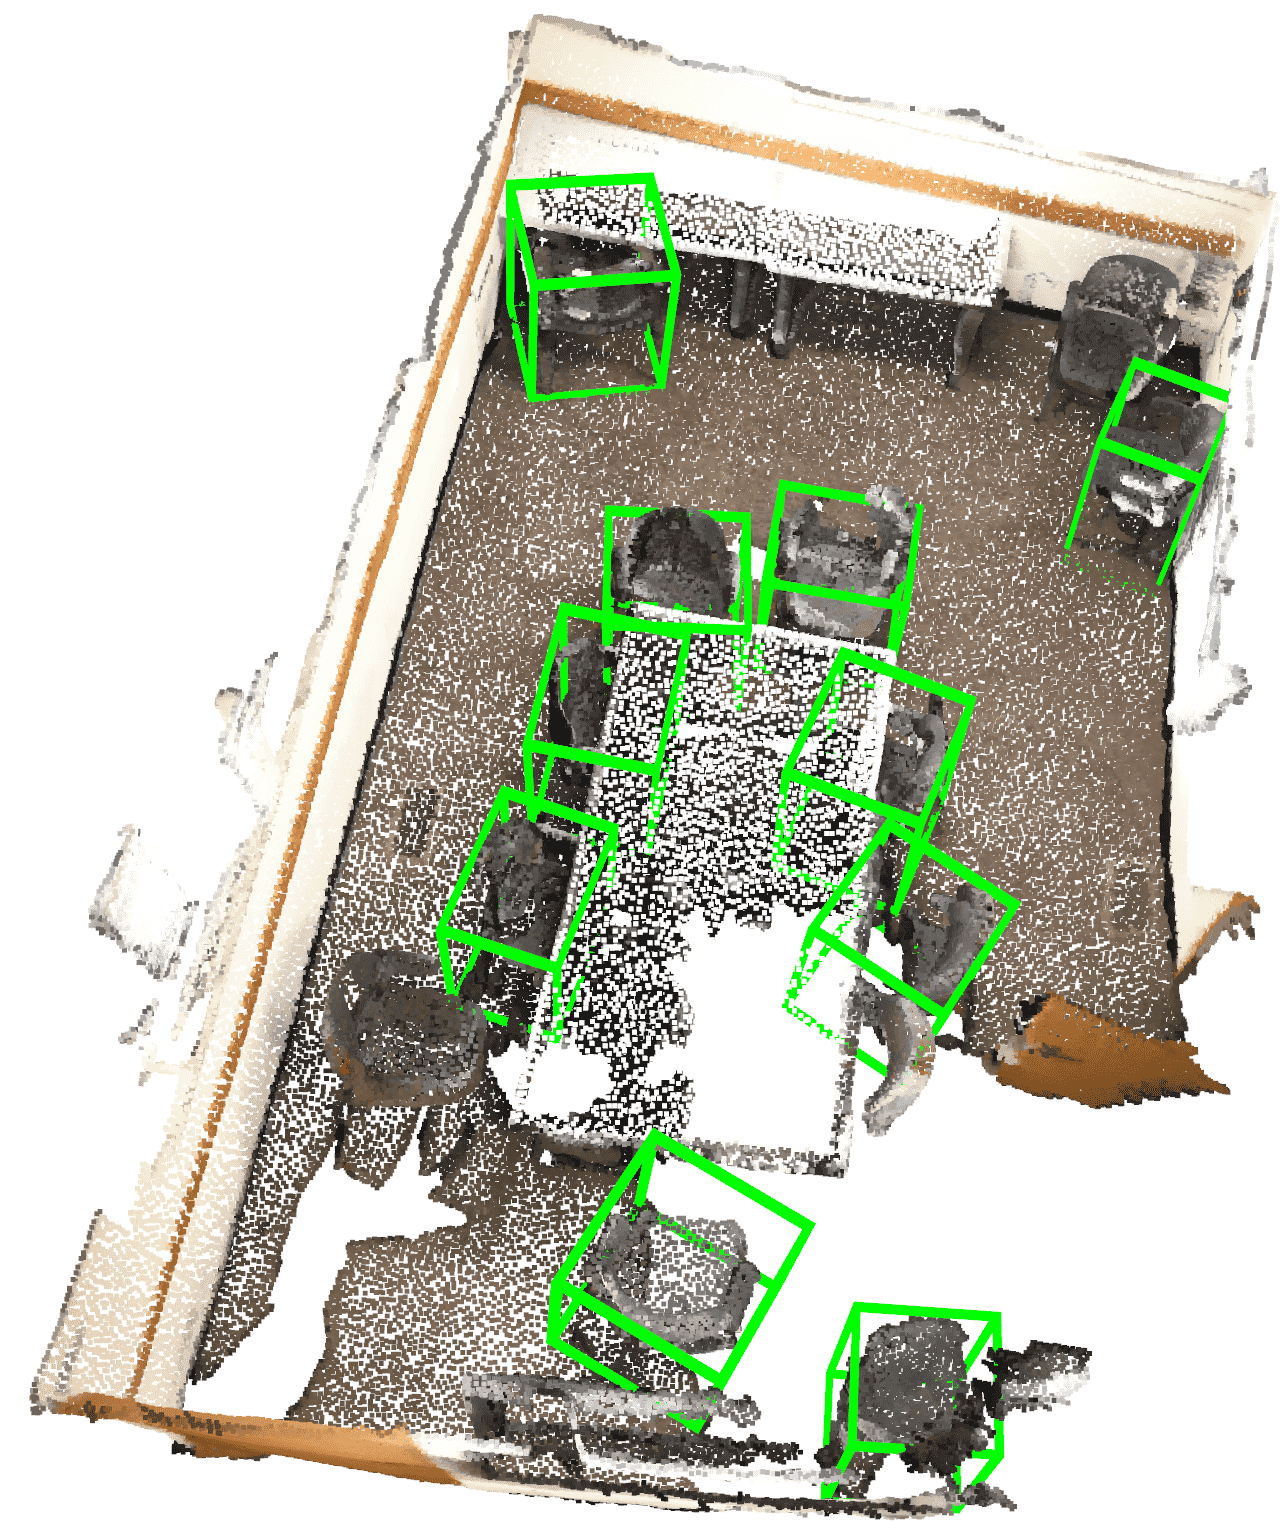
\includegraphics[height=3.3cm]{images/scan2cad-cad-consac.png}
          \caption{CONSAC\cite{CONSAC}}
          \label{fig:scan2cad_cad-consac}
      \end{subfigure}
      \begin{subfigure}{0.18\textwidth}
        \centering
        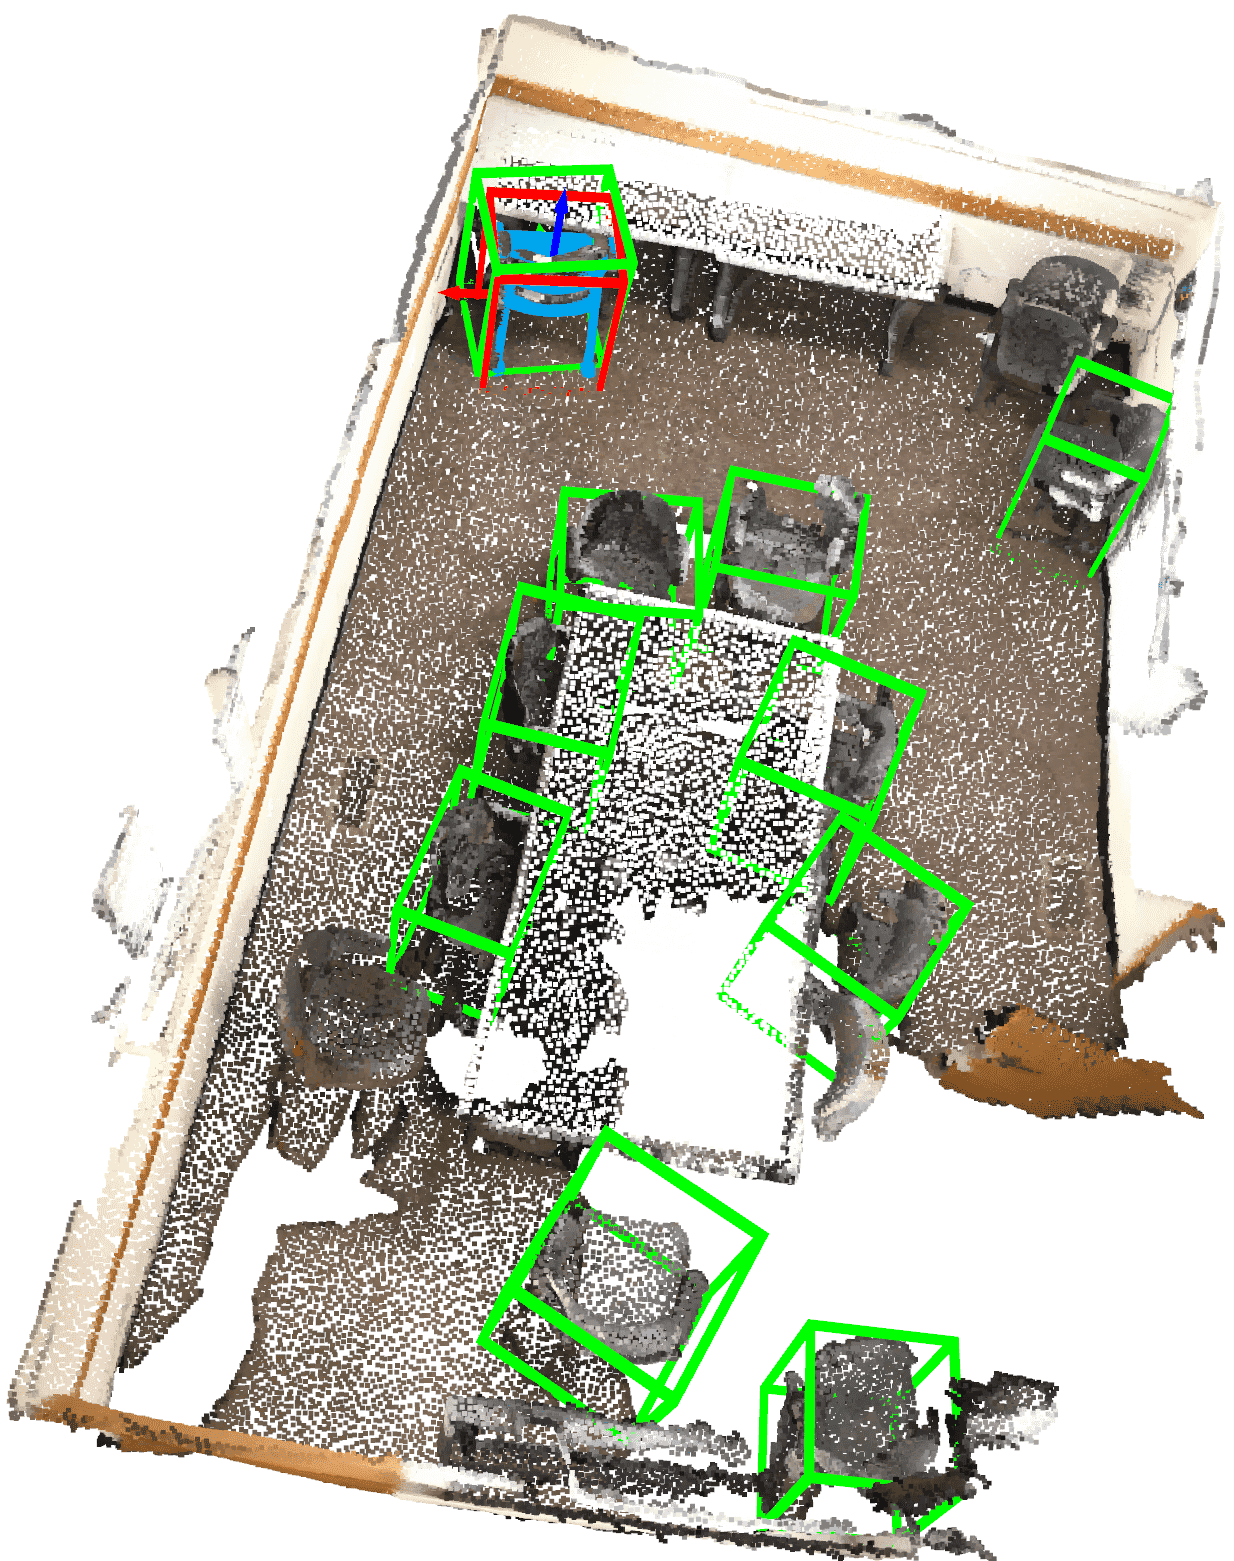
\includegraphics[height=3.3cm]{images/scan2cad-cad-teaser.png}
          \caption{TEASER\cite{TEASER}}
          \label{fig:scan2cad_cad-teaser}
      \end{subfigure}
      % \begin{subfigure}{0.15\textwidth}
      %   \centering
      %   \includegraphics[height=3cm]{scan2cad-cad-ransac.png}
      %     \caption{RANSAC}
      %     \label{fig:scan2cad_cad-ransac}
      % \end{subfigure}
      \caption{\textbf{Scan2CAD 结果。} (a) 通过匹配 PREDATOR \cite{PREDATOR} 特征得到的输入对应关系。内点和离群点分别用绿色和红色显示。 (b) 我们的聚类结果用不同颜色显示(仅显示内点)。在 (c-g) 中,我们将估计的姿态用红色框显示,将真实姿态用绿色框显示。我们的方法 (c) 正确地对齐了 8 个实例。T-Linkage (d) 和 CONSAC (f) 未能配准任何实例。Progressive-X (e) 配准了 3 个实例。TEASER (g) 注册了一个实例。}
\label{fig:Scan2CAD-cadresult}
\end{figure*}

\begin{figure*}[ht]
    \centering
    \begin{subfigure}{0.4\textwidth}
        \centering
        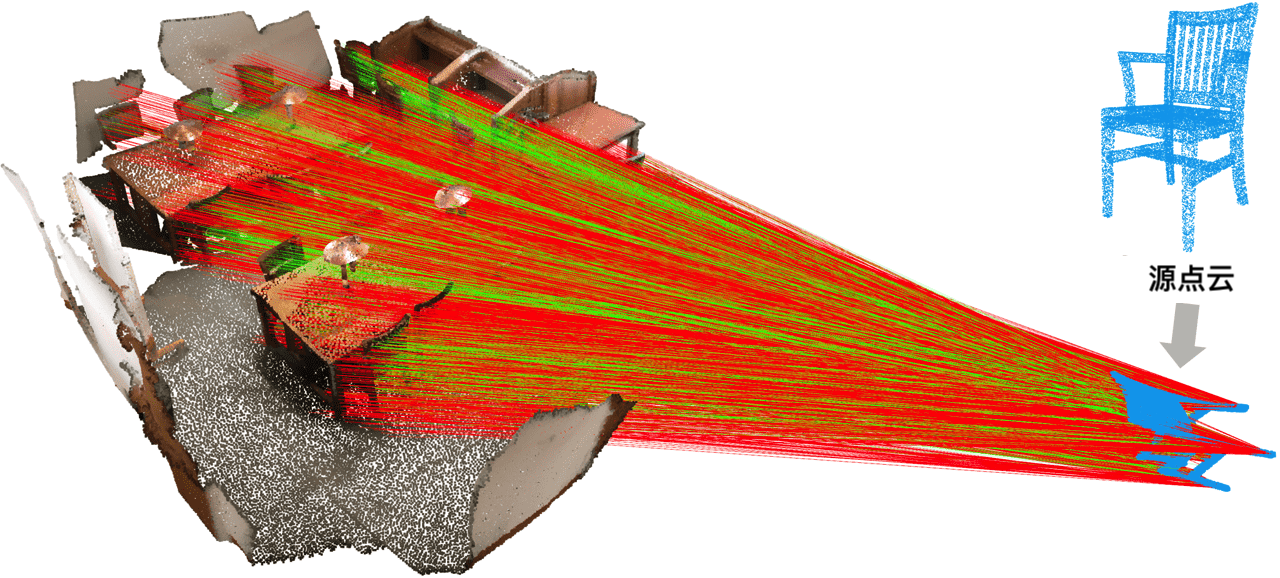
\includegraphics[height=2.8cm]{images/scan2cad-cad-input-corrs1.png}
          \caption{Input correspondences}
          \label{fig:scan2cad_cad-input-corrs1}
      \end{subfigure}
      \begin{subfigure}{0.45\textwidth}
        \centering
        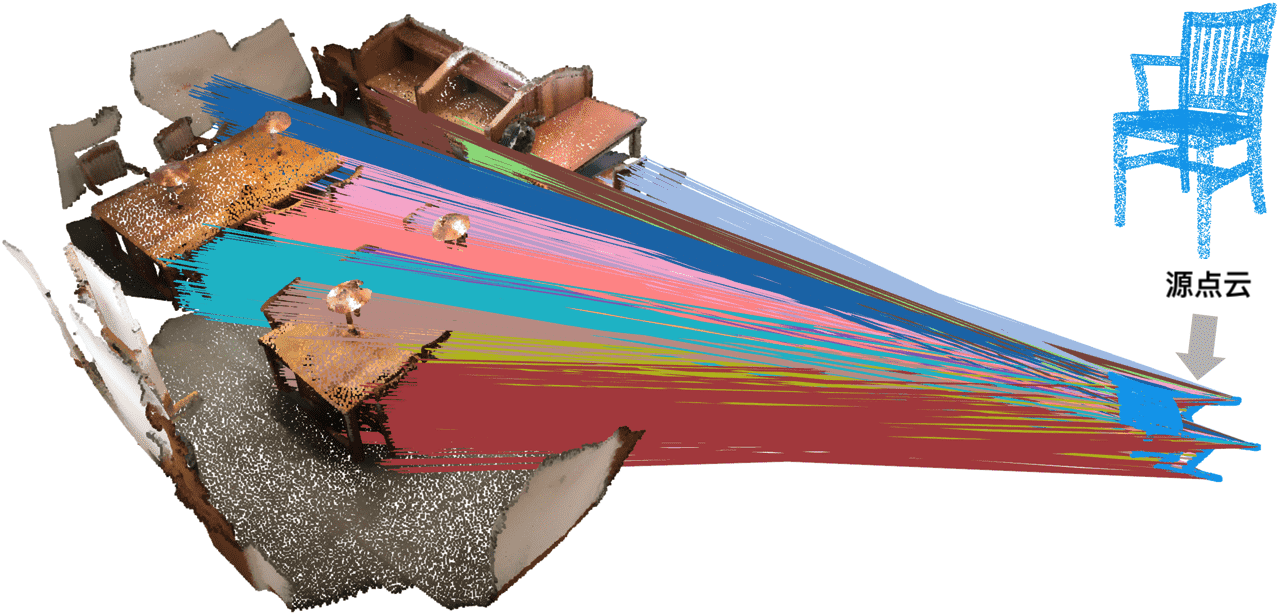
\includegraphics[height=2.8cm]{images/scan2cad-cad-cluster-corrs1.png}
          \caption{Our clustering result}
          \label{fig:scan2cad_cad-cluster-corrs1}
      \end{subfigure}


      \begin{subfigure}{0.18\textwidth}
        \centering
        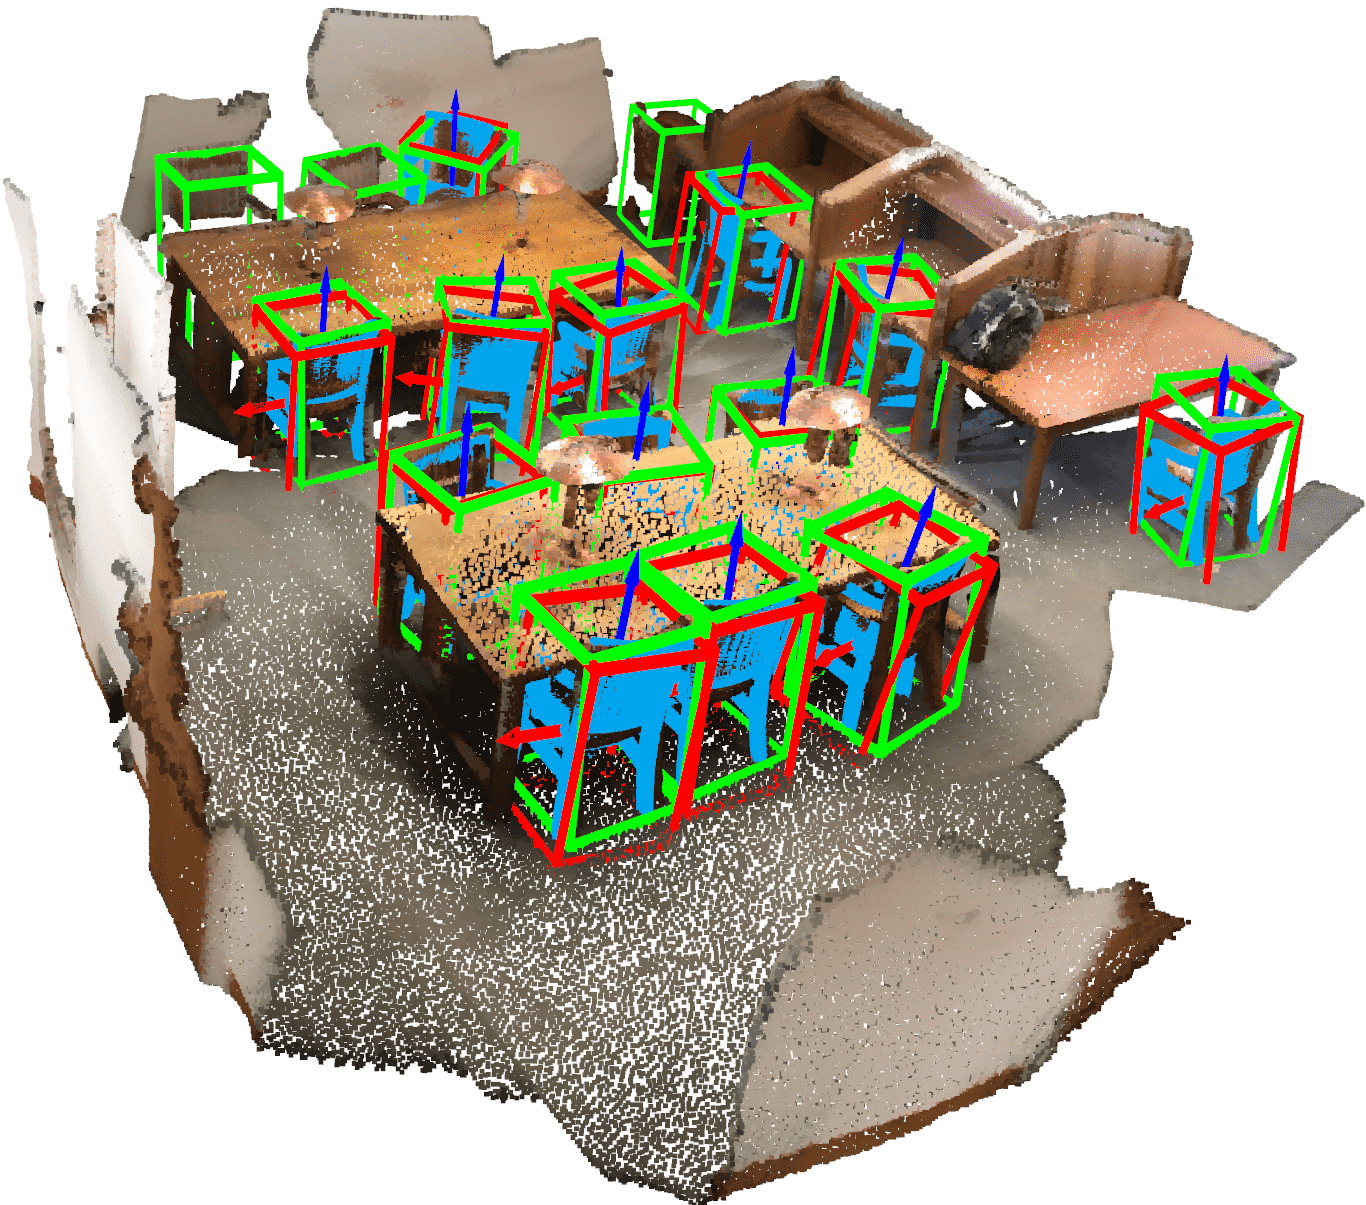
\includegraphics[height=2.8cm]{images/scan2cad-cad-ours1.png}
          \caption{Ours}
          \label{fig:scan2cad_cad-result1}
      \end{subfigure}
      \begin{subfigure}{0.18\textwidth}
        \centering
        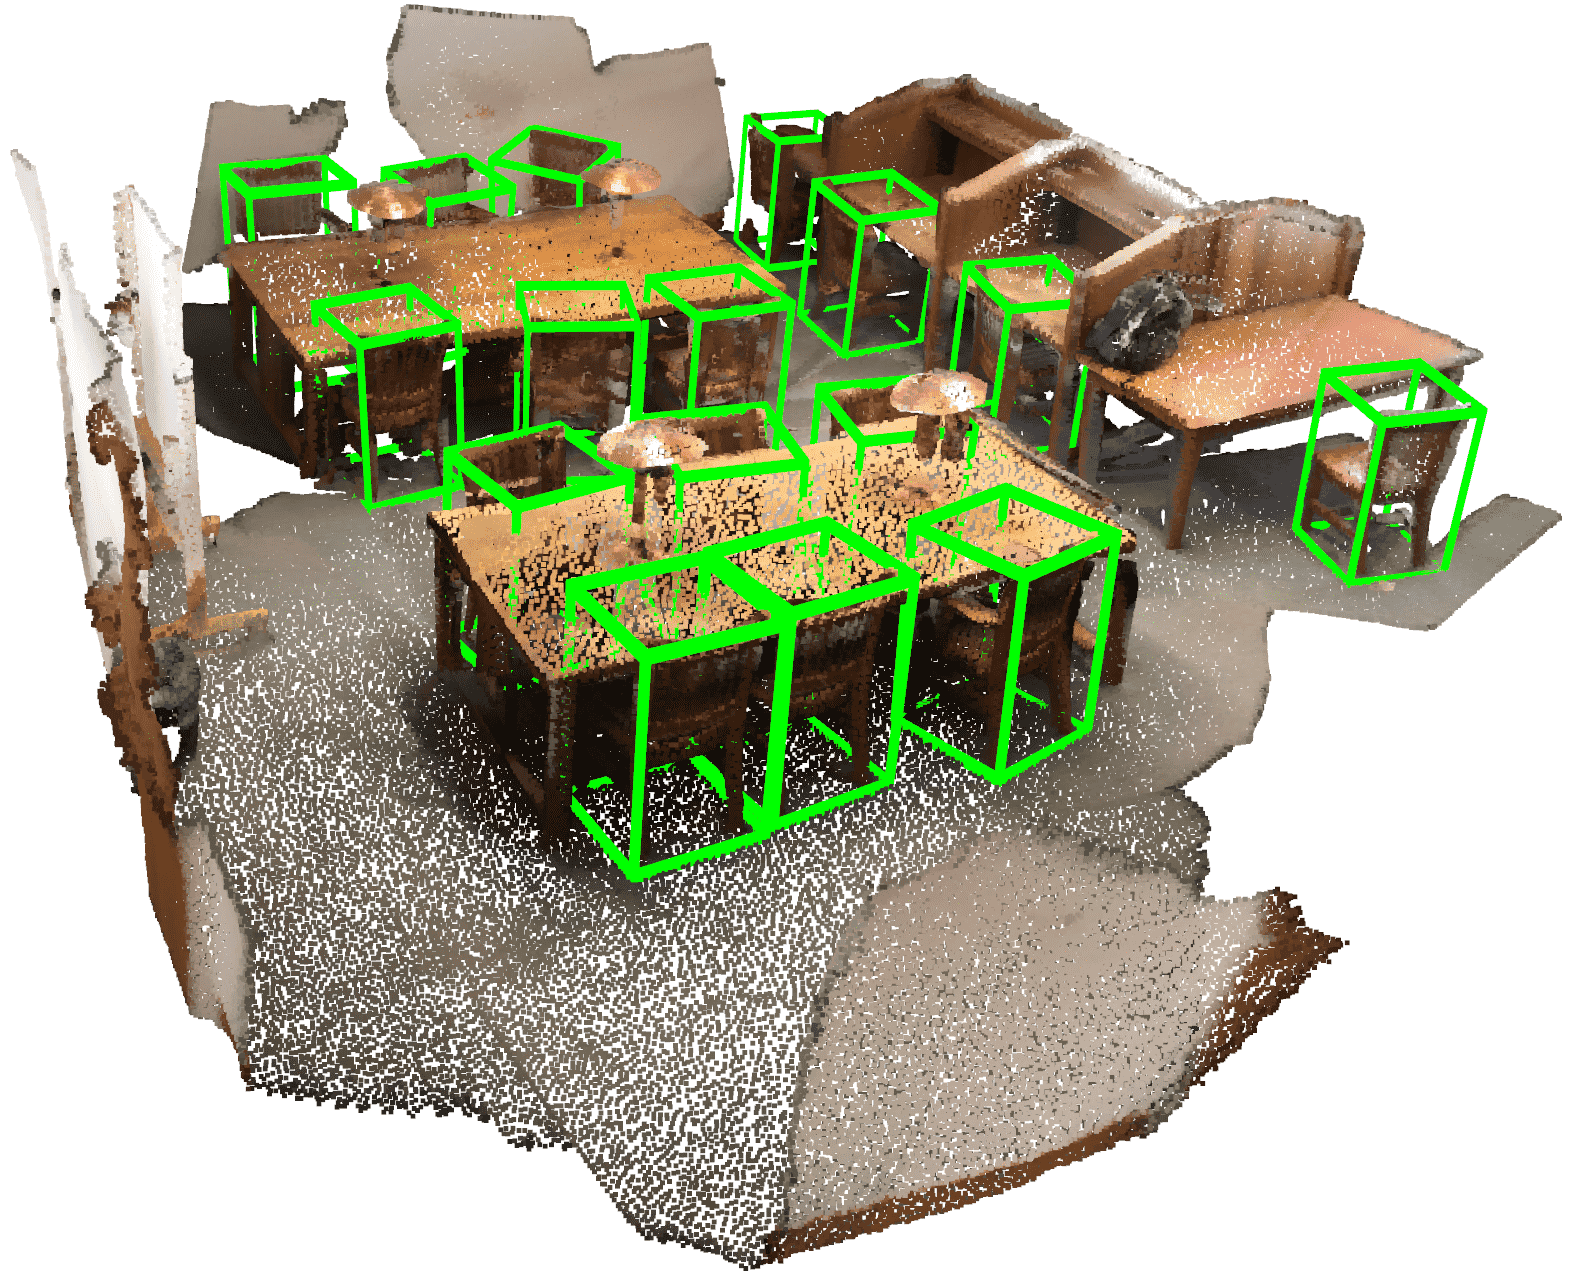
\includegraphics[height=2.8cm]{images/scan2cad-cad-tlinkage1.png}
          \caption{T-linkage\cite{Tlinkage}}
          \label{fig:scan2cad_cad-tlinkage1}
      \end{subfigure}
      \begin{subfigure}{0.2\textwidth}
        \centering
        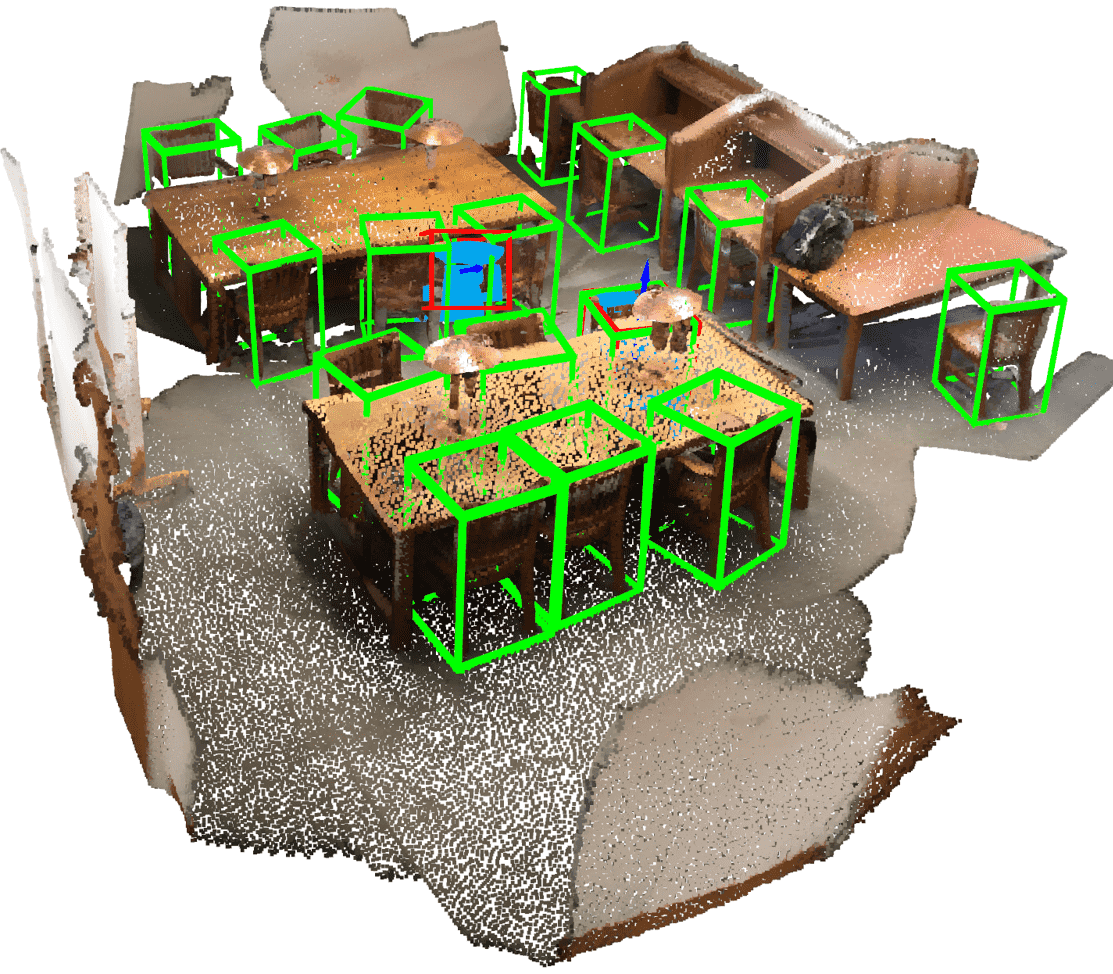
\includegraphics[height=2.8cm]{images/scan2cad-cad-progx1.png}
          \caption{Progressive-X\cite{ProgressiveX}}
          \label{fig:scan2cad_cad-prox1}
      \end{subfigure}
      \begin{subfigure}{0.18\textwidth}
        \centering
        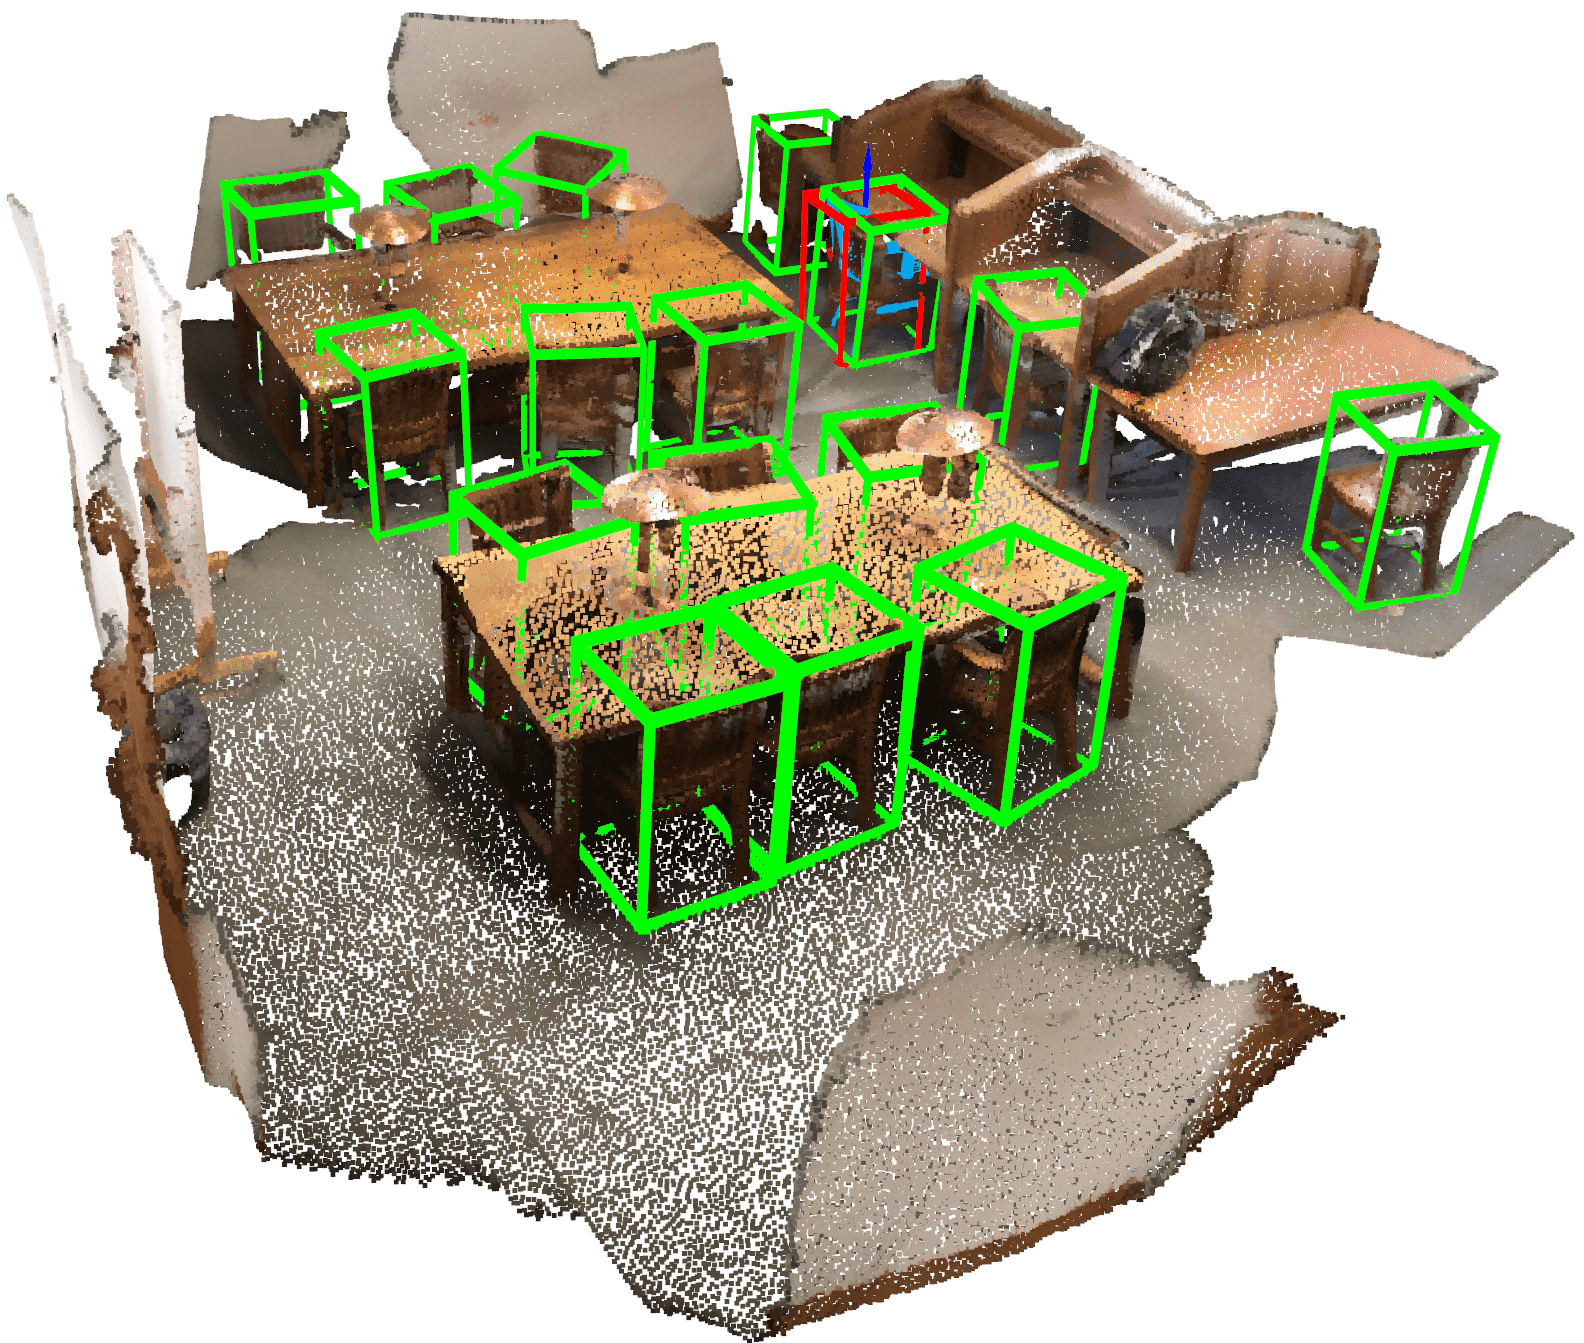
\includegraphics[height=2.8cm]{images/scan2cad-cad-consac1.png}
          \caption{CONSAC\cite{CONSAC}}
          \label{fig:scan2cad_cad-consac1}
      \end{subfigure}
      \begin{subfigure}{0.18\textwidth}
        \centering
        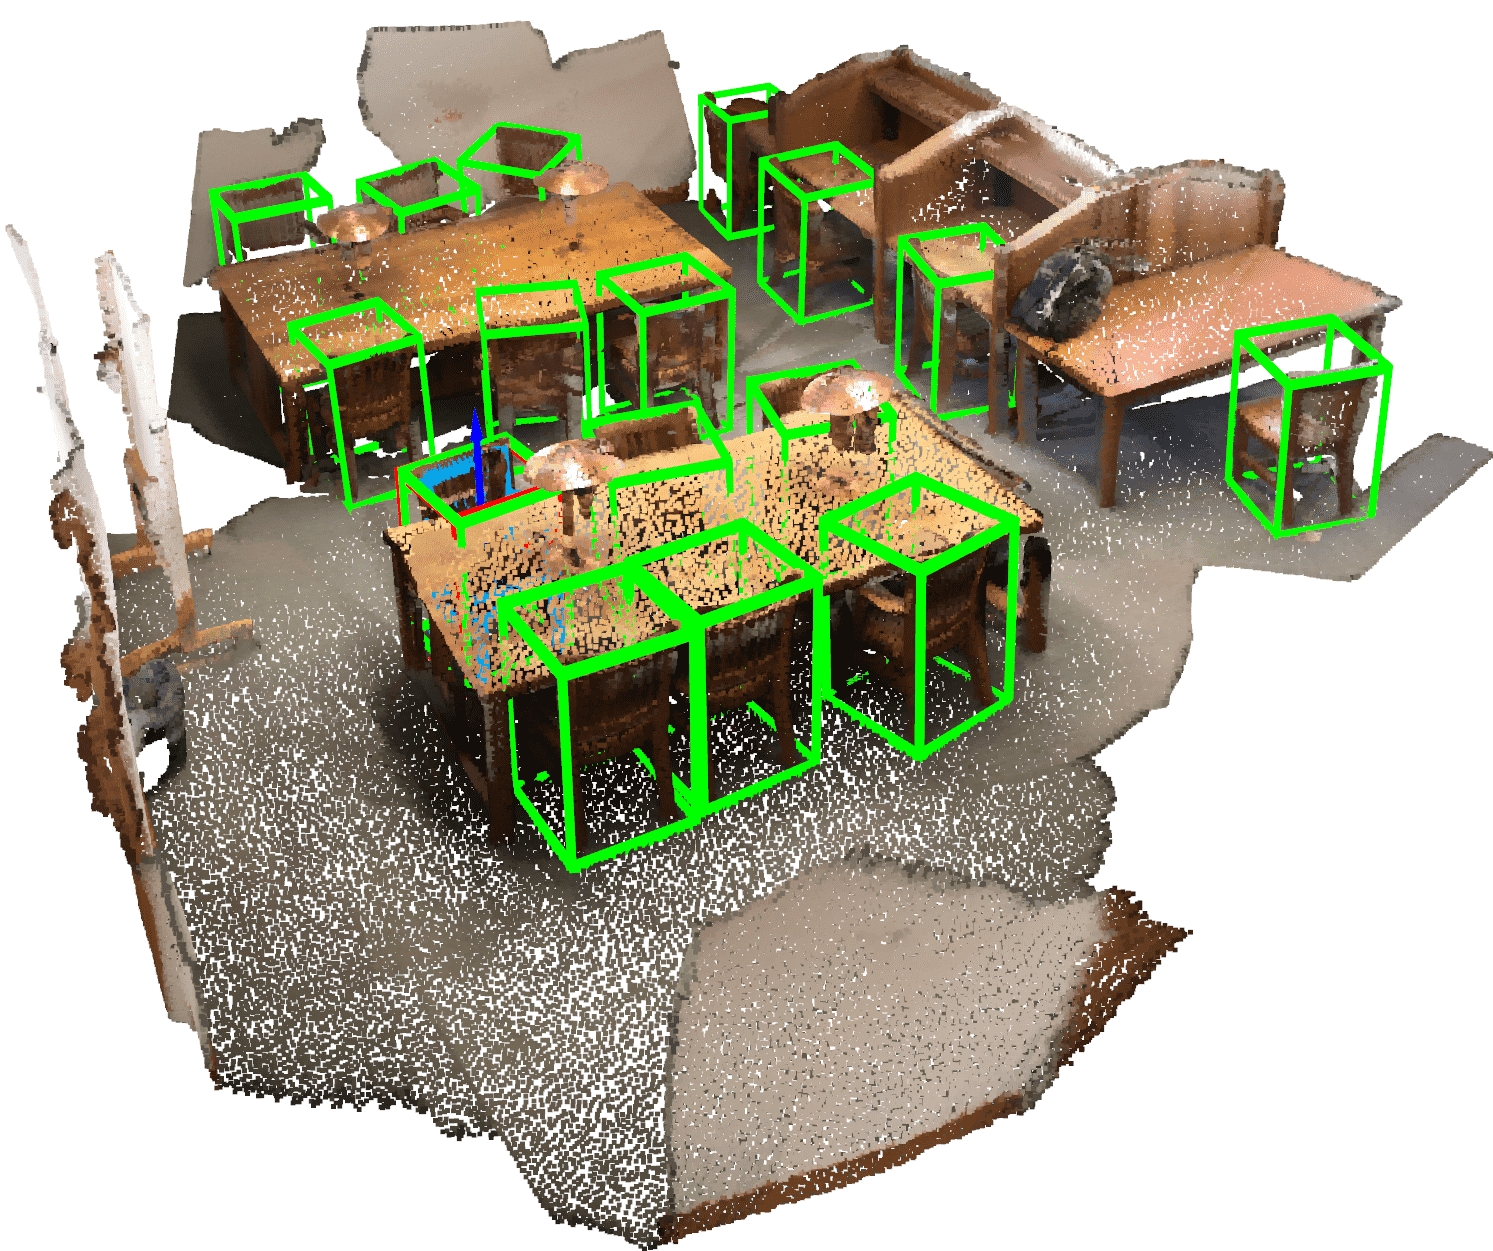
\includegraphics[height=2.8cm]{images/scan2cad-cad-teaser1.png}
          \caption{TEASER\cite{TEASER}}
          \label{fig:scan2cad_cad-teaser1}
      \end{subfigure}
      % \begin{subfigure}{0.18\textwidth}
      %   \centering
      %   \includegraphics[height=2.5cm]{scan2cad-cad-ransac1.png}
      %     \caption{RANSAC}
      %     \label{fig:scan2cad_cad-ransac1}
      % \end{subfigure}
      \caption{\textbf{Scan2CAD 结果。} 我们的方法 (c) 在 16 个椅子中配准了 13 个实例。Progressive-X (e) 配准了 2 个实例,但其中一个的姿态误差较大。CONSAC (f) 和 TEASER (g) 都配准了一个实例。T-Linkage (d) 未能配准任何实例。}
\label{fig:Scan2CAD-cadresult1}
\end{figure*}



\paragraph{基于特征匹配的对应关系}
在此测试中,我们使用 PREDATOR\cite{PREDATOR} 和 D3Feat\cite{D3Feat} 特征匹配来获得点对应关系。这两个特征模型都是在合成数据上训练的。结果显示在表 \ref{tab:realcorr} 中。请注意,这两个特征都产生了超过 $90\%$ 的高离群点比例。在这样一个具有挑战性的情况下,我们的方法在鲁棒性和效率方面仍然表现良好,且明显优于现有方法。使用 D3Feat 的结果要比使用 PREDATOR 的结果差得多。原因不仅是因为更多的离群点,而且我们在检查结果时发现缺少内点。我们在图 \ref{fig:predatormm} 中展示了一些结果。

\begin{table}[ht]
    \scriptsize
        \centering
            \begin{tabular}{ccccc} 
                \toprule
                \textbf{Metric}& MHR$\left( \% \right) \uparrow $& MHP$\left( \% \right) \uparrow $& MHF1$\left( \% \right) \uparrow $ & Time$\left( s \right) \downarrow $\\
                \hline
                & \multicolumn{4}{c}{PREDATOR ( estimated outlier ratio : $94.32\%$)} \\
                \hline
                T-Linkage & 0.19 & 0.54 & 0.27 & 43.46 \\
                Progressive-X & 15.90 & 31.01 & 18.98 & 86.39 \\
                CONSAC & 0.1 & 0.07 & 0.08 & 7.65 \\
                \textbf{Ours} &\textbf{53.39} & \textbf{61.44} & \textbf{51.80} & \textbf{1.28/0.48} \\
                \hline
                
                &\multicolumn{4}{c}{D3Feat ( estimated outlier ratio : $99.30\%$)} \\
                \hline
                %\hline
                % \textbf{metric} & MHR$\left( \% \right) \uparrow $ & RRE$\left( \degree \right) \downarrow $ & RTE$\left( m \right) \downarrow $ & t$\left( s \right) \downarrow $\\
                %\hline
                %\hline
                T-Linkage & 0.07 & 0.29 & 0.1 & 56.37  \\
                Progressive-X & 4.29 & 15.28 & 5.94 & 87.22 \\
                CONSAC & 0.13 & 0.04 & 0.05 & 9.53 \\
                \textbf{Ours} & \textbf{16.98} & \textbf{27.05} & \textbf{17.91} & \textbf{0.68/0.30} \\
                \bottomrule
        \end{tabular}
        \caption{使用特征匹配在合成数据上生成对应点的结果。部分结果可在图 \ref{fig:predatormm} 中进行可视化。}
        % \caption{Results on synthetic data using feature matching to generate correspondences.$\uparrow$ means the larger the better, while $\downarrow$ indicates the contrary. The running time on CPU/GPU of our method is presented. Some results are visualized in Figure \ref{fig:predatormm}.}
        \label{tab:realcorr}
        \end{table}
    
    
    
\begin{table}[h]
  \scriptsize 
  \centering
            %\resizebox{.95\columnwidth}{!}{
    \begin{tabular}{ccccc} %& $50\%~70\%$ & $70\%~90\%$
    \toprule
    \textbf{Metric}& MHR$\left( \% \right) \uparrow $& MHP$\left( \% \right) \uparrow $& MHF1$\left( \% \right) \uparrow $ & Time$\left( s \right) \downarrow $ \\
    \hline
    & \multicolumn{4}{c}{PREDATOR( estimated outlier ratio : $76.44\%$)} \\
    \hline
    T-Linkage & 2.46 & 3.79 & 2.71 & 1655.0 \\
    Progressive-X & 11.58 & 6.86 & 7.87 & 26.32\\
    CONSAC & 2.66 & 0.35 & 0.62 & 21.35\\
    \textbf{Ours} & \textbf{31.63} & \textbf{29.23} & \textbf{27.04} & \textbf{1.46/0.51} \\
    \hline
                    
    &\multicolumn{4}{c}{ D3Feat ( estimated outlier ratio :  $97.25\%$)} \\
    \hline
    T-Linkage & 0.04 & 0.22 & 0.06 & 2178.43 \\
    Progressive-X & \textbf{0.67} & \textbf{0.30} & \textbf{0.4} & 28.48 \\
    CONSAC & 0 & 0 & 0 & 21.88 \\
    \textbf{Ours} & 0.29 & 0.04 & 0.07 & \textbf{2.13/0.89} \\
  \bottomrule
  \end{tabular}
    \caption{在Scan2CAD数据集上点的结果。}
    \label{tab:Scan2CAD-cad}
\end{table}

\begin{table}[ht]
    \centering
\scriptsize
    %\resizebox{.95\columnwidth}{!}{
    \begin{tabular}{ccccc}
      \toprule
        Box Size& MHR$\left( \% \right) \uparrow $ & MHP $\left( \% \right) \uparrow $ & MHF1$\left( \% \right) \uparrow $& Time$\left( s \right) \downarrow $ \\
        \midrule  
        1.5 ($94.50\%$) & 40.58 & 12.61 & 16.64 & 0.63  \\
        2 ($95.97\%$) & 37.43 & 8.85 & 12.35 & 1.37  \\
        4 ($98.73\%$)& 7.25 & 6.28 & 4.92 & 3.86  \\
        \bottomrule
    \end{tabular}
    \caption{在 Scan2CAD 数据集上使用不同大小的边界框进行特征匹配的结果。估计的异常值比率在框大小后的括号内列出。最后一列列出了 GPU 时间。
    }
    \label{tab:biggerbox}
\end{table}



\section{基准数据集}
Scan2CAD\cite{Scan2cad} 是一个基准数据集,它将 ShapeNet\cite{ShapeNet} CAD 模型与 ScanNet\cite{ScanNet} 点云中的对象实例对齐。部分扫描有多个已对齐的 CAD 模型和标注的姿态。我们选择那些包含多个 CAD 模型的扫描作为目标点云,并从 CAD 模型中采样源点云进行测试。我们为配准测试生成了 173 个样本,其中大多数样本包含 $2 \sim 5$ 个实例。
请注意,在每个点云中,Scan2CAD 中仅标注了部分实例。这意味着我们无法使用部分标注的姿态正确评估性能,如准确率和召回率。为解决这个问题,我们仅在目标点云中标注的物体的真实边界框内匹配点以生成对应关系。同样,我们使用 PREDATOR\cite{PREDATOR} 和 D3Feat\cite{D3Feat} 进行点匹配,两者都是使用 Scan2CAD 数据集中的 1028 个训练样本和 187 个验证样本进行微调的。
% 对于每个目标点,我们
% 选择具有最相似特征的源点作为对应关系。
结果如表 \ref{tab:Scan2CAD-cad} 所示。我们的方法在使用 PREDATOR 时明显优于现有方法。请注意,当使用 D3Feat 时,所有方法的性能都很差。在仔细检查结果后,我们发现原因不仅是高异常值比率(约 $97.25\%$),而且在使用 D3Feat 时,即使特征匹配仅限于目标点云中的真实边界框内,内点也不足。一些结果如图 \ref{fig:Scan2CAD-cadresult} 和图 \ref{fig:Scan2CAD-cadresult1} 所示。
我们还通过将边界框扩大 $1.5\times, 2.0\times$ 和 $4.0\times$ 来评估我们方法的性能。当框大小调整为 $4\times$ 时,目标点云几乎是原始扫描。基于 PREDATOR 特征的结果如表 \ref{tab:biggerbox} 所示。当包含更多背景点时,特征匹配变得更具挑战性,产生高度噪声的对应关系,这使得我们方法的 MHF1(平均命中 F1)显著降低。
  
\section{真实场景测试}
我们使用一个 RGB-D 相机(Intel D455)捕捉一系列点云,这些点云表示了桌子上的一堆物体,并将我们的算法应用于将某个特定物体的 3D 扫描与目标 RGB-D 扫描中的多个实例进行对齐。由于颜色信息可用,我们使用 SIFT 特征生成 3D 点对应关系。然后我们应用我们的算法提取每个物体的姿态。图 \ref{fig:app} 显示了一些结果。尽管桌子上摆满了不同的物体,但我们的方法几乎能实时地(每帧约 $0.2$ 秒)正确地将源 3D 扫描与多达十几个实例进行对齐。更多结果可以在补充材料中找到。

\begin{figure}[h]
  \centering   
  \begin{subfigure}{0.3\textwidth}
    \centering
    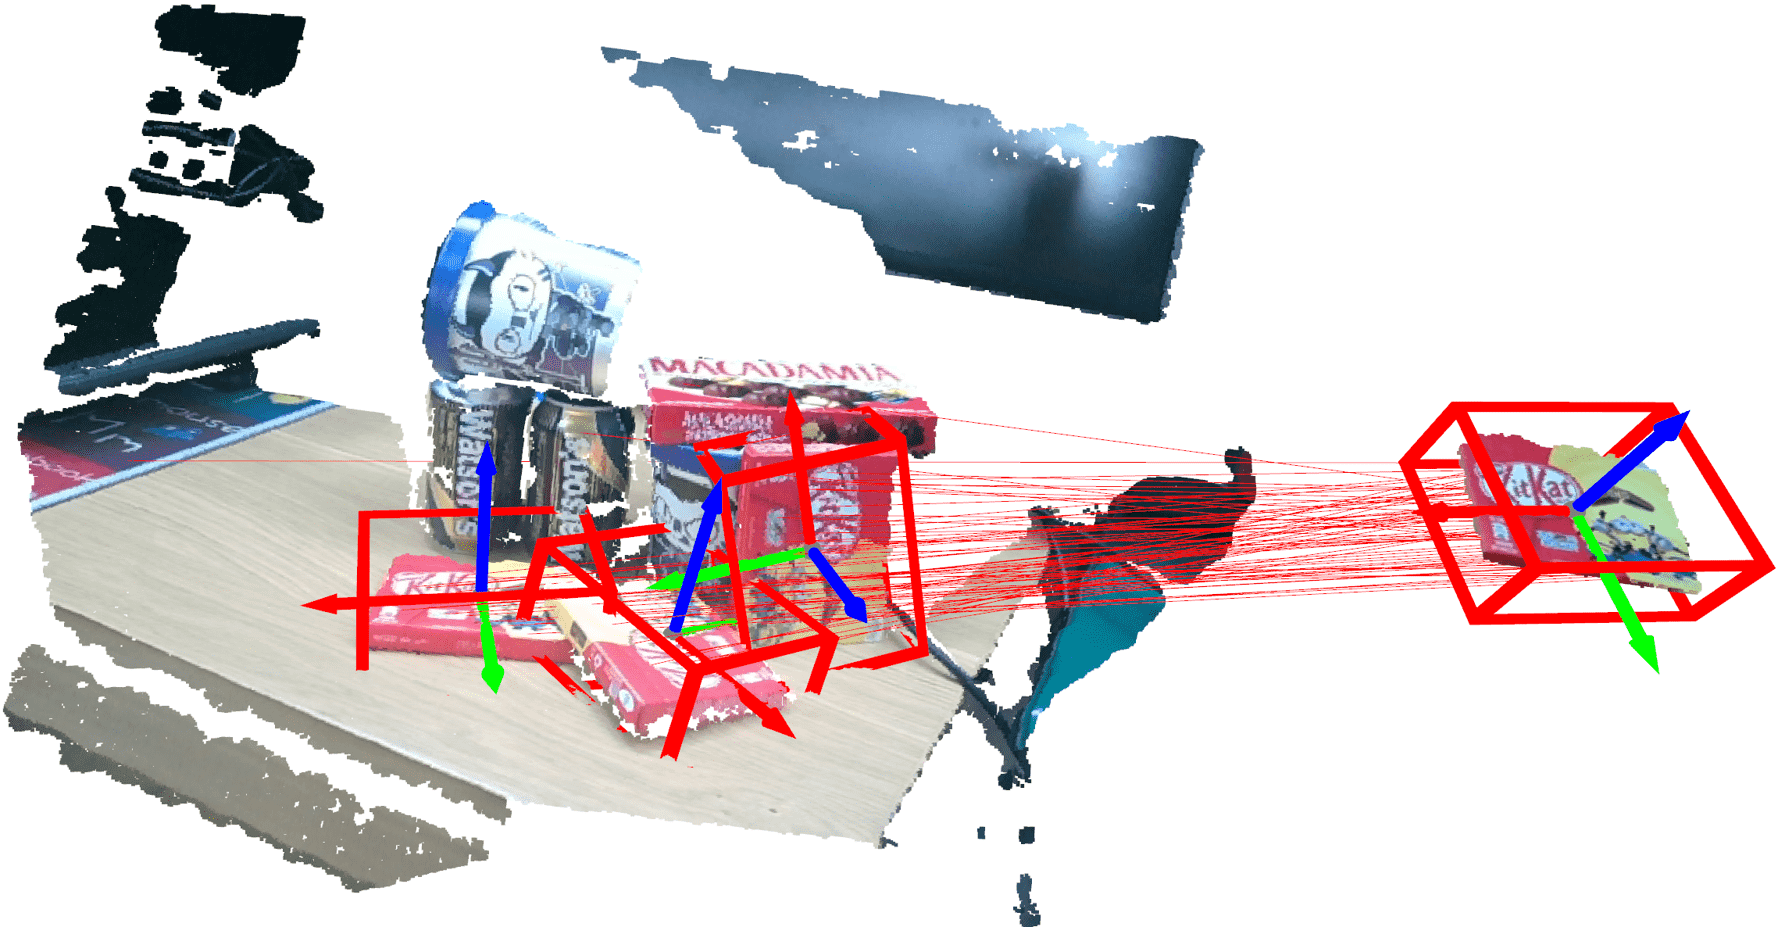
\includegraphics[height=2.cm]{images/real1.png}
      \caption{Kitkat}
      \label{fig:real1}
  \end{subfigure}
  \begin{subfigure}{0.3\textwidth}
    \centering
    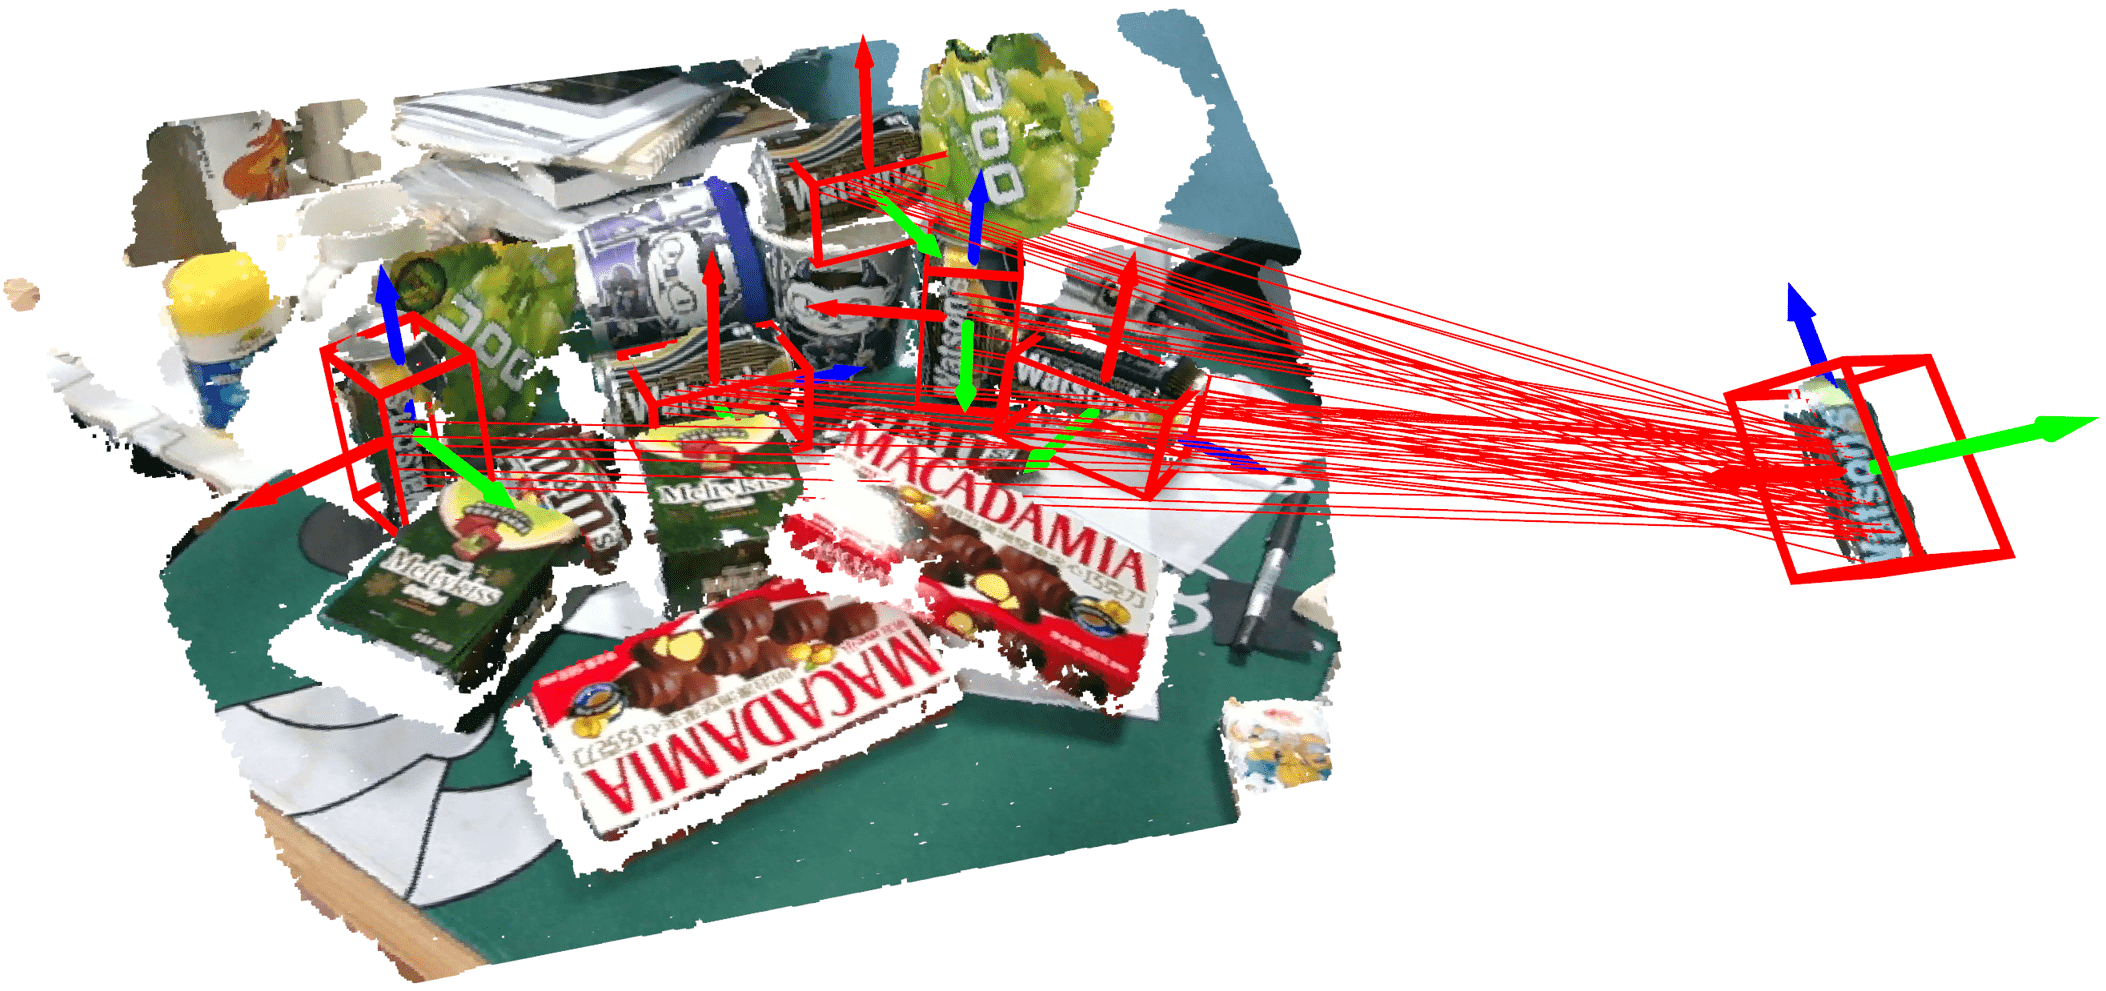
\includegraphics[height=2.cm]{images/real2.png}
      \caption{Watson}
      \label{fig:real2}
  \end{subfigure}


    \begin{subfigure}{0.3\textwidth}
    \centering
    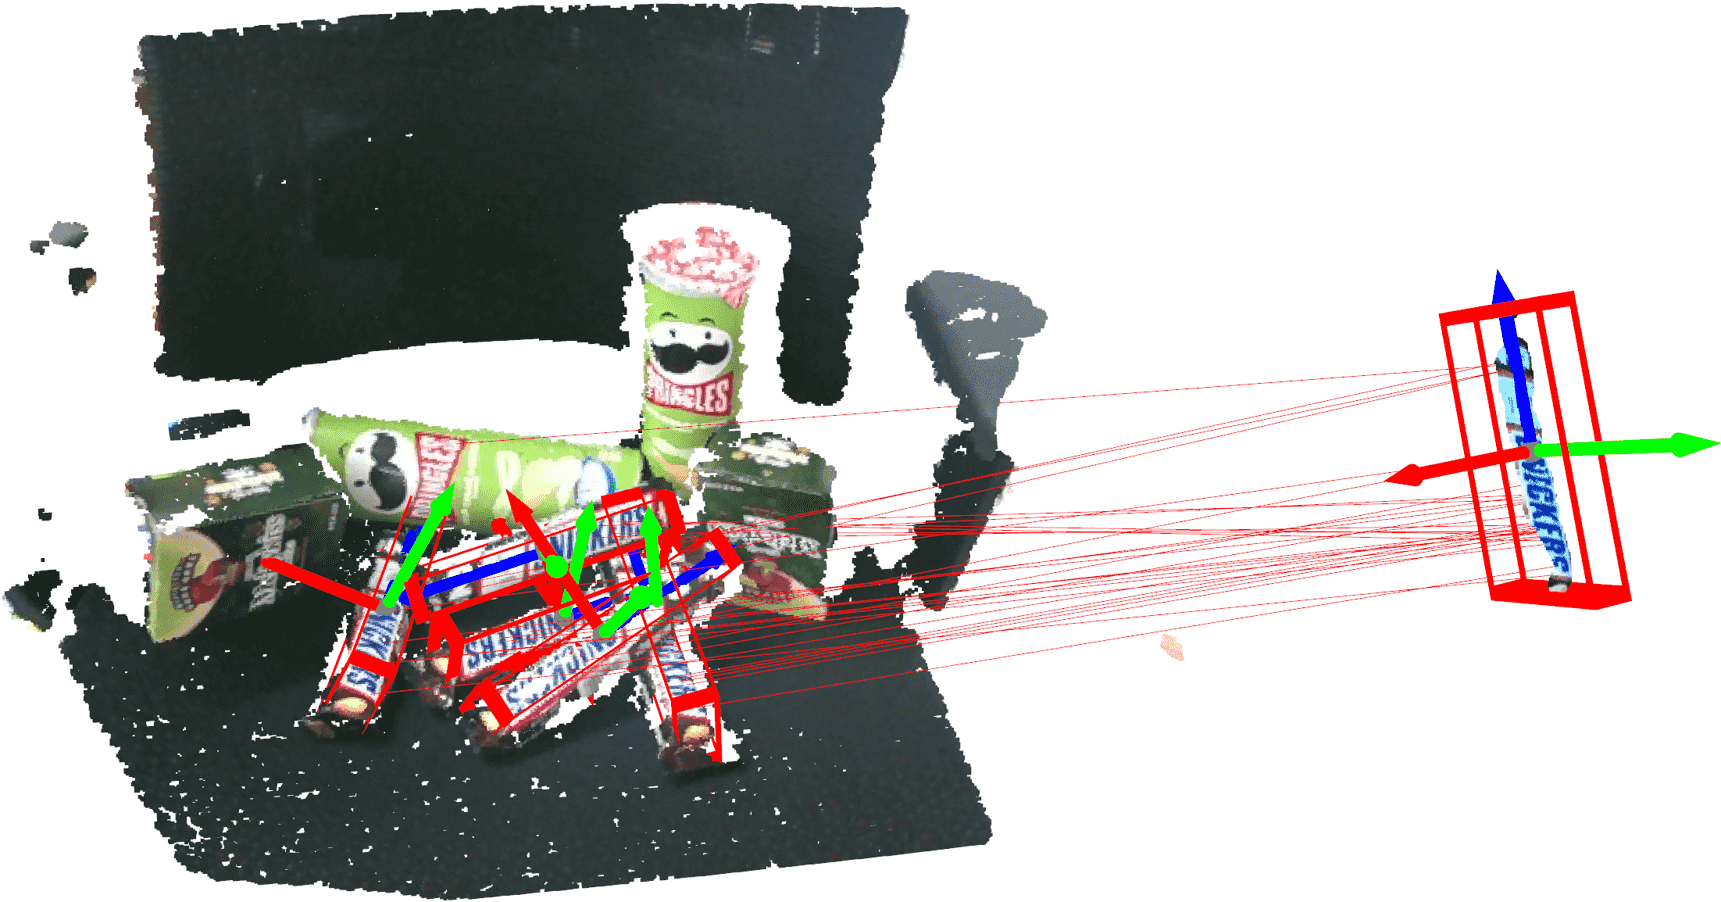
\includegraphics[height=2.cm]{images/real3.png}
      \caption{Snickers}
      \label{fig:real3}
  \end{subfigure}
  \begin{subfigure}{0.3\textwidth}
    \centering
    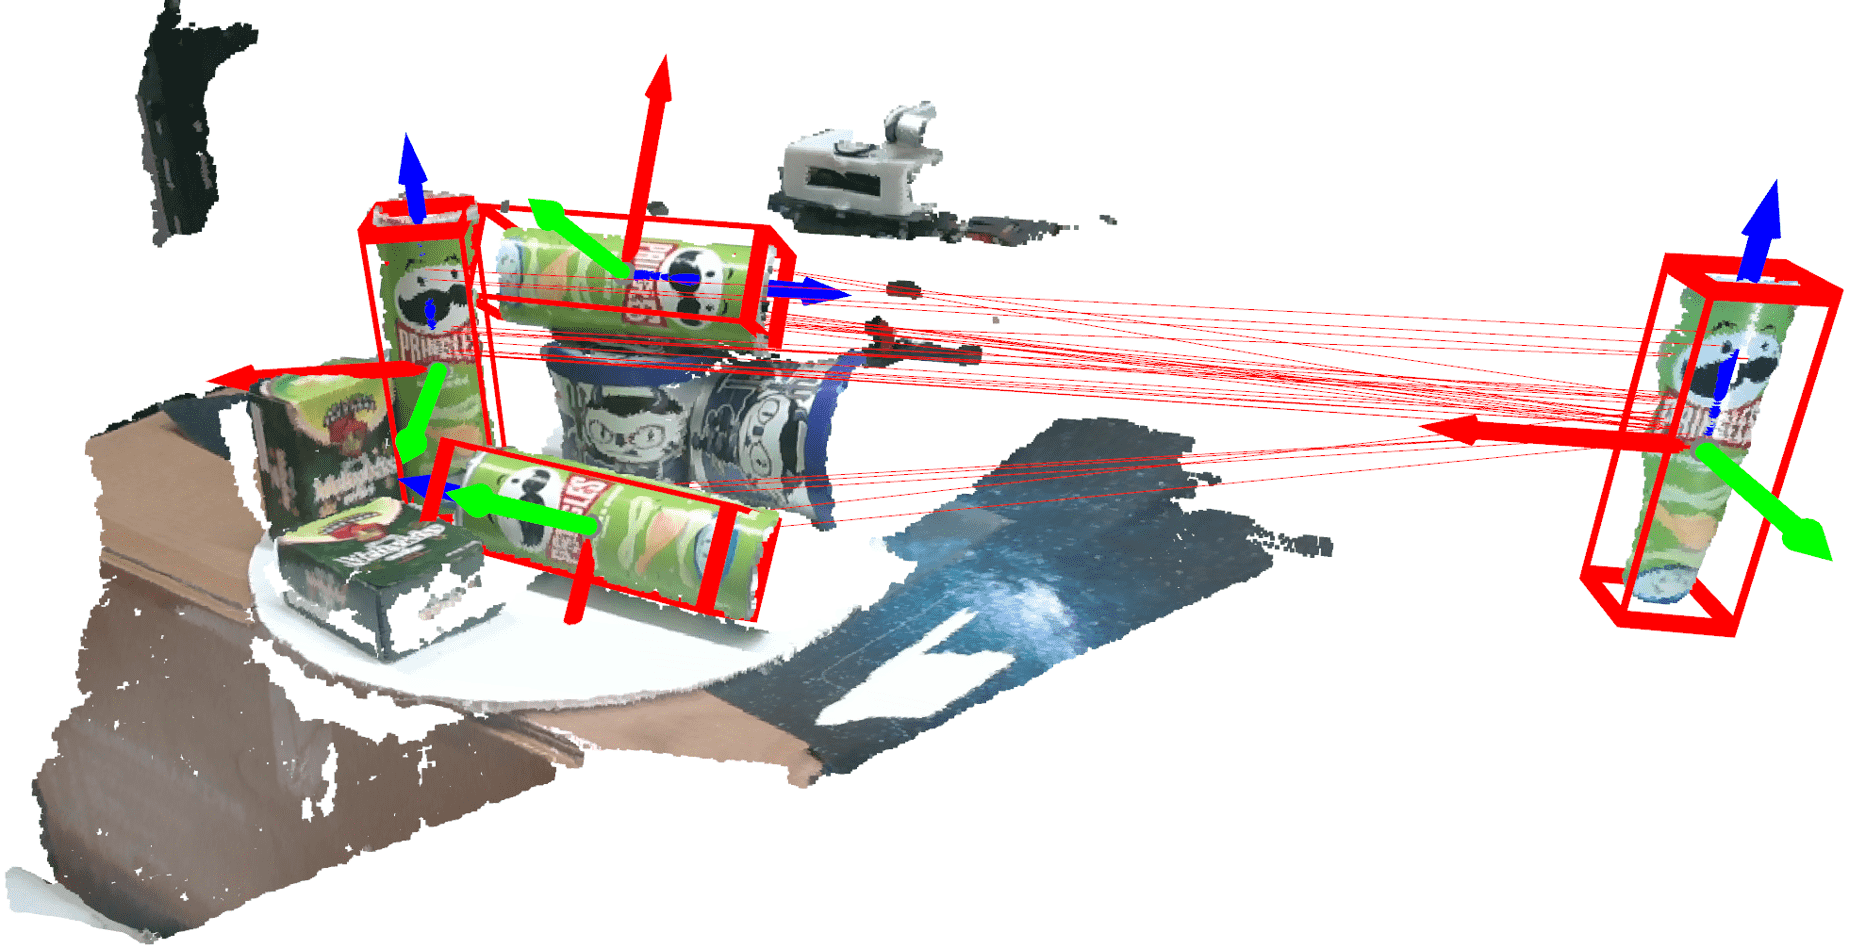
\includegraphics[height=2.cm]{images/real4.png}
      \caption{Crisp}
      \label{fig:real4}
  \end{subfigure}
  \caption{实际测试基于 RGB-D 扫描。源点云是从单个物体的深度扫描中提取的。目标点云是从相机视点捕获的深度扫描构建的。}
\label{fig:app}
\end{figure}


\chapter{局限性}
我们方法的性能依赖于点对应关系的质量。不幸的是,我们发现使用诸如 D3Feat 和 PREDATOR 这样的最先进的 3D 特征产生的对应关系不令人满意,尽管它们在一些基准测试中表现良好。为了提高对应关系的质量,我们必须为实验中的每个数据集训练这些特征。即使这样做,异常值比率仍然很高,有时某些实例的内点会丢失(特别是在使用 D3Feat 时),这会显著降低召回率,正如实验所示。因此,3D 特征是一个需要显著改进的瓶颈。另一个局限性是距离不变性对于噪声点云来说是一个弱规则,有时不足以排除接近内点的异常值,这也可能降低我们方法的性能。一种可能的解决方案是在端到端学习管线中寻找更好的不变性“特征”来表示每个对应关系,如 \cite{PointDSC}。
\chapter{结论}
在本文中,我们讨论了多实例 3D 配准的新颖任务。我们发现距离不变性矩阵的列向量编码了与对应关系相关的实例的丰富信息。基于这个观察,我们通过聚类算法将对应关系高效地聚类到不同的组中,并通过多次迭代来优化结果。在合成、基准和实际数据集上的结果表明,我们的方法在鲁棒性、准确性和效率方面明显优于现有方法。尽管我们的解决方案仍然远非完美,正如所讨论的那样,但我们希望我们的工作能激发对这一主题的未来研究。
% 后置部分
\backmatter

% 结论:在结论相应的 TeX 文件处进行结论部分的撰写
% %%
% The BIThesis Template for Bachelor Paper Translation
%
% 北京理工大学毕业设计(论文) —— 使用 XeLaTeX 编译
%
% Copyright 2020-2023 BITNP
%
% This work may be distributed and/or modified under the
% conditions of the LaTeX Project Public License, either version 1.3
% of this license or (at your option) any later version.
% The latest version of this license is in
%   http://www.latex-project.org/lppl.txt
% and version 1.3 or later is part of all distributions of LaTeX
% version 2005/12/01 or later.
%
% This work has the LPPL maintenance status `maintained'.
%
% The Current Maintainer of this work is Feng Kaiyu.
%
% Compile with: xelatex -> biber -> xelatex -> xelatex
%%

\begin{conclusion}
  % 结论部分尽量不使用 \subsection 二级标题,只使用 \section 一级标题

  % 这里插入一个参考文献,仅作参考
  本文结论……。\cite{李成智2004飞行之梦}

  \textcolor{blue}{结论作为毕业设计(论文)正文的最后部分单独排写,但不加章号。结论是对整个论文主要结果的总结。在结论中应明确指出本研究的创新点,对其应用前景和社会、经济价值等加以预测和评价,并指出今后进一步在本研究方向进行研究工作的展望与设想。结论部分的撰写应简明扼要,突出创新性。阅后删除此段。}

  \textcolor{blue}{结论正文样式与文章正文相同:宋体、小四;行距:22 磅;间距段前段后均为 0 行。阅后删除此段。}
\end{conclusion}

% 参考文献:如无特殊需要,参考文献相应的 TeX 文件无需改动,添加参考文献请使用 BibTeX 的格式
%   添加至 misc/ref.bib 中,并在正文的相应位置使用 \cite{xxx} 的格式引用参考文献
%%
% The BIThesis Template for Bachelor Paper Translation
%
% 北京理工大学毕业设计(论文) —— 使用 XeLaTeX 编译
%
% Copyright 2020-2023 BITNP
%
% This work may be distributed and/or modified under the
% conditions of the LaTeX Project Public License, either version 1.3
% of this license or (at your option) any later version.
% The latest version of this license is in
%   http://www.latex-project.org/lppl.txt
% and version 1.3 or later is part of all distributions of LaTeX
% version 2005/12/01 or later.
%
% This work has the LPPL maintenance status `maintained'.
%
% The Current Maintainer of this work is Feng Kaiyu.
%
% Compile with: xelatex -> biber -> xelatex -> xelatex
%%

\begin{bibprint}
  \printbibliography[heading=none]
\end{bibprint}

% 附录:在附录相应的 TeX 文件处进行附录部分的撰写
% %%
% The BIThesis Template for Bachelor Paper Translation
%
% 北京理工大学毕业设计(论文) —— 使用 XeLaTeX 编译
%
% Copyright 2020-2023 BITNP
%
% This work may be distributed and/or modified under the
% conditions of the LaTeX Project Public License, either version 1.3
% of this license or (at your option) any later version.
% The latest version of this license is in
%   http://www.latex-project.org/lppl.txt
% and version 1.3 or later is part of all distributions of LaTeX
% version 2005/12/01 or later.
%
% This work has the LPPL maintenance status `maintained'.
%
% The Current Maintainer of this work is Feng Kaiyu.
%
% Compile with: xelatex -> biber -> xelatex -> xelatex
%%

\begin{appendices}
  附录相关内容…

  % 这里示范一下添加多个附录的方法:

  \section{\LaTeX 环境的安装}
  \LaTeX 环境的安装。

  \section{BIThesis 使用说明}
  BIThesis 使用说明。

  \textcolor{blue}{附录是毕业设计(论文)主体的补充项目,为了体现整篇文章的完整性,写入正文又可能有损于论文的条理性、逻辑性和精炼性,这些材料可以写入附录段,但对于每一篇文章并不是必须的。附录依次用大写正体英文字母 A、B、C……编序号,如附录 A、附录 B。阅后删除此段。}

  \textcolor{blue}{附录正文样式与文章正文相同:宋体、小四;行距:22 磅;间距段前段后均为 0 行。阅后删除此段。}

\end{appendices}



\end{document}
